%%%%%%%%%%%%%%%%%%%%%%%%%%%%%%%%%%%%%%%%%%%%%%%%%%%
%% Tutorial Visualisasi Data Menggunakan Seaborn   %%
%% Penyusun: Sandy Herho (sandyherho.github.io)   %%
%% License: MIT License                          %%
%%%%%%%%%%%%%%%%%%%%%%%%%%%%%%%%%%%%%%%%%%%%%%%%%%%

\documentclass[a4paper,11pt]{book}
\usepackage[T1]{fontenc}
\usepackage[utf8]{inputenc}
\usepackage{lmodern}
\usepackage{hyperref}
%%%%%%%%%%%%%%%%%%%%%%%%%%%%%%%%%%%%%%%%%%%%%%%%%%%%%%%%%
% Sumber: http://en.wikibooks.org/wiki/LaTeX/Hyperlinks %
%%%%%%%%%%%%%%%%%%%%%%%%%%%%%%%%%%%%%%%%%%%%%%%%%%%%%%%%%
\usepackage{hyperref}
\usepackage{graphicx}
\usepackage[bahasa]{babel}
\usepackage{float}
\usepackage{fancyvrb}
\usepackage{longtable}
\usepackage{tabularx}
% listing
\usepackage{listings}
\usepackage{color}
\usepackage{float}
\usepackage{verbatim}
\usepackage{alltt}
\usepackage{caption}



%New colors defined below
\definecolor{codegreen}{rgb}{0,0.6,0}
\definecolor{codegray}{rgb}{0.5,0.5,0.5}
\definecolor{codepurple}{rgb}{0.58,0,0.82}
\definecolor{backcolour}{rgb}{0.95,0.95,0.92}

%Code listing style named "mystyle"
\lstdefinestyle{mystyle}{
  backgroundcolor=\color{backcolour},   commentstyle=\color{codegreen},
  keywordstyle=\color{magenta},
  numberstyle=\tiny\color{codegray},
  stringstyle=\color{codepurple},
  basicstyle=\footnotesize,
  breakatwhitespace=false,         
  breaklines=true,                 
  captionpos=b,                    
  keepspaces=true,                 
  numbers=left,                    
  numbersep=5pt,                  
  showspaces=false,                
  showstringspaces=false,
  showtabs=false,                  
  tabsize=2
}

%"mystyle" code listing set
\lstset{style=mystyle}
%listing

%%%%%%%%%%%%%%%%%%%%%%%%%%%%%%%%%%%%%%%%%%%%%%%%%%%%%%%%%%%%%%%%%%%%%%%%%%%%%%%%
% 'dedication' environment: To add a dedication paragraph at the start of book %
% Source: http://www.tug.org/pipermail/texhax/2010-June/015184.html            %
%%%%%%%%%%%%%%%%%%%%%%%%%%%%%%%%%%%%%%%%%%%%%%%%%%%%%%%%%%%%%%%%%%%%%%%%%%%%%%%%
\newenvironment{dedication}
{
   \cleardoublepage
   \thispagestyle{empty}
   \vspace*{\stretch{1}}
   \hfill\begin{minipage}[t]{0.66\textwidth}
   \raggedright
}
{
   \end{minipage}
   \vspace*{\stretch{3}}
   \clearpage
}

%%%%%%%%%%%%%%%%%%%%%%%%%%%%%%%%%%%%%%%%%%%%%%%%

%%%%%%%%%%%%%%%%%%%%%%%%%%%%%%%%%%%%%%%%%%%%%%%%
\makeatletter
\renewcommand{\@chapapp}{}% Not necessary...
\newenvironment{chapquote}[2][2em]
  {\setlength{\@tempdima}{#1}%
   \def\chapquote@author{#2}%
   \parshape 1 \@tempdima \dimexpr\textwidth-2\@tempdima\relax%
   \itshape}
  {\par\normalfont\hfill--\ \chapquote@author\hspace*{\@tempdima}\par\bigskip}
\makeatother

%%%%%%%%%%%%%%%%%%%%%%%%%%%%%%%%%%%%%%%%%%%%%%%%%%%
% Halaman awal dalam buku yang memuat hal - hal seperti:Judul Buku, sub-judul, dan nama penuyusun.
%%%%%%%%%%%%%%%%%%%%%%%%%%%%%%%%%%%%%%%%%%%%%%%%%%%

% Judul Buku dan Sub-Judul
\title{\Huge \textbf{Tutorial Visualisasi Data} \\ \huge Menggunakan Seaborn}
% Author
\author{\textsc{Sandy Hardian Susanto Herho}\thanks{\url{https://sandyherho.github.io/}}}


\begin{document}

\frontmatter
\maketitle

%%%%%%%%%%%%%%%%%%%%%%%%%%%%%%%%%%%%%%%%%%%%%%%%%%%%%%%%%%%%%%%
% Dedikasi Buku %
%%%%%%%%%%%%%%%%%%%%%%%%%%%%%%%%%%%%%%%%%%%%%%%%%%%%%%%%%%%%%%%
\begin{dedication}
Untuk Guru - Guru saya: \mbox{\textbf{M.R. Syahputra}}, \mbox{\textbf{D.E. Irawan}}, dan \mbox{\textbf{F.R. Fajary}}\\
\end{dedication}

%%%%%%%%%%%%%%%%%%%%%%%%%%%%%%%%%%%%%%%%%%%%%%%%%%%%%%%%%%%%%%%%%%%%%%%%
% Auto-generated table of contents, list of figures and list of tables %
%%%%%%%%%%%%%%%%%%%%%%%%%%%%%%%%%%%%%%%%%%%%%%%%%%%%%%%%%%%%%%%%%%%%%%%%
\tableofcontents
%\listoffigures
%\listoftables

\mainmatter

%%%%%%%%%%%
% Kata Pengantar %
%%%%%%%%%%%
\chapter*{Kata Pengantar}
Seaborn merupakan pustaka visualisasi data pada lingkungan Python bersifat sumber terbuka yang berlisensi BSD dan dibangun di atas pustaka matplotlib. Seaborn akan mempermudah kita sebagai analis data untuk memproduksi visualisasi yang indah tanpa kostumisasi rumit seperti yang kita hadapi pada matplotlib. Seaborn awalnya diperkenalkan Michael askom\footnote{\url{https://www.cns.nyu.edu/~mwaskom/}}, yang kala itu merupakan seorang mahasiswa doktoral neurosains di Universitas Stanford,  untuk memvisualisasikan data untuk analisis jaringan saraf pada awal tahun 2014 silam. Saat ini seaborn telah memasuki versi stabil 0.9.0, dan akan terus dikembangkan oleh komunitasnya yang cukup besar. 

Tutorial ini sendiri dimaksudkan untuk membantu pembaca untuk memahami dasar - dasar penggunaan seaborn untuk memvisualisasikan analisis statistik sederhana yang biasa dihadapi oleh mahasiswa tingkat dua di seluruh jurusan perguruan tinggi di Indonesia pada praktikum matakuliah statistika. Diharapkan tutorial ini dapat dijadikan alternatif penyelesaian tugas praktikum yang umumnya menggunakan piranti lunak berbayar yang tidak mendidik, seperti SPSS, MS Excel, Matlab, dll.Untuk memahami tutorial ini, pembaca diharapkan telah terbiasa dengan sintaks - sintaks dalam bahasa pemrograman Python dan mengenal dasar - dasar penggunaan matplotlib.

Saya memohon maaf jika tutorial ini punya banyak sekali kekurangan, karena pada hakikatnya saya bukan bekerja sebagai analis data profesional yang bekerja di persuahaan besar, yang menggunakan Python sebagai rutinitas hariannya. Pada dasarnya tutorial ini hanya merupakan catatan - catatan pembelajaran yang saya himpun dari berbagai sumber, utamanya dari dokumentasi resmi\footnote{\url{http://seaborn.pydata.org/}}, sehingga tentunya jika ada yang tidak jelas dalam tutorial ini atau ingin memperdalam bagian tertentu, pembaca dapat mengunjungi laman tersebut.

Tutorial ini juga bersifat sumber terbuka, karena dituliskan dengan menggunakan \LaTeX{} dan berlisensi milik publik (\textit{copy-left}), sehingga para pembaca dapat mengopi dan mengubahnya, bahkan untuk kepentingan komersil sekalipun, secara cuma - cuma di \url{https://github.com/sandyherho/buku_seaborn}.

Akhir kata, semoga tutorial singkat dapat membantu dan saya menanti dengan tangan terbuka kolaborasi pembelajaran berbasis kode terbuka di laman GitHub saya.  

\mbox{}\\
%\mbox{}\\
\noindent Sandy H.S. Herho \\\\
\noindent \textbf{\textit{College Park, MD.}}

%%%%%%%%%%%%%%%%
% ISI %
%%%%%%%%%%%%%%%%
\chapter{Pendahuluan}

Pada bidang keilmuan analisis data, cara terbaik untuk memperoleh pemahaman yang mendalam terhadap suatu data adalah dengan cara memvisualisasikannya. Representasi visual data mempermudah pemahaman otak kita sebagai manusia (berbeda dengan komputer yang lebih memahami angka dibandingkan visual), sehingga memungkinkan kita untuk mengeksplorasi data tersebut secara lebih jauh. 

Sebagai pengguna setia Python, tentunya kita telah terbiasa menggunakan pustaka matplotlib guna memvisualisasikan data dalam keseharian kita. Seaborn sesungguhnya tidaklah jauh berbeda dibandingkan matplotlib, sebab seaborn dibangun di atas matplotlib sebagai pustaka fondasi utama-nya. 

Plot - plot rumit yang sukar dikerjakan oleh para analis data pemula dalam matplotlib dapat dengan mudah dikerjakan dalam seaborn. Bahkan terkadang dapat ddikerjakan dengan menggunakan satu baris perintah saja (seperti yang akan kita sama - sama lihat dalam bab - bab berikutnya).

Seaborn memberikan solusi terhadap dua permasalahan berikut yang umumnya dihadapi oleh para analis data pemula ketika menggunakan matplotlib:
\begin{itemize}
	\item Kerumitan penggunakan parameter - parameter standar dalam matplotlib.
	\item Kerumitan matplotlib ketika bekerja dengan \textit{data frame}.
\end{itemize}

Sebagaimana yang telah saya bahas di atas, seaborn dibangun dengan matplotlib sebagai pustaka fondasi utama-nya. Seaborn dalam hal ini merupakan pelengkap matplotlib, bukan pengganti. Namun, seaborn dilengkapi oleh fitur - fitur penting yang mempermudah kita dalam memvisualisasikan data. Berikut ini merupakan fitur - fitur tersebut:
\begin{itemize}
    \item Tema \textit{built-in} yang mempercantik tampilan grafis matplotlib.
    \item Visualisasi data univariat dan bivariat.
    \item Penyesuaian dan visualisasi model regresi linier.
    \item Plot data deret waktu (\textit{time-series}) statistik.
    \item Dapat bekerja dengan baik bersama dengan berbagai jenis struktur data pada numpy dan Pandas.
\end{itemize}

Dalam banyak kasus, kita masih akan menggunakan matplotlib untuk menghasilkan plot - plot sederhana. Oleh karena itu, pengetahuan tentang matplotlib sangat dibutuhkan untuk mengubah plot - plot standar dalam seaborn.

\chapter{Pengaturan Lingkungan Komputasi}
Pada bagian ini kita akan membahas proses penyesuaian lingkungan komputasi yang dibutuhkan untuk melakukan visualisasi data dengan menggunakan seaborn. Kita memulainya dengan melakukan instalasi seaborn.

Untuk pengguna Python standar kita dapat menggunakan \textit{pip installer} dengan menjalankan perintah berikut di Terminal (GNU/Linux dan MacOS) atau PowerShell (MS Windows):
\begin{verbatim}
    pip install seaborn
\end{verbatim}
Namun saya sangat menyarankan agar kita menggunakan distribusi Anaconda yang akan berguna bagi para analis data kedepannya. Distribusi ini dapat diunduh secara gratis di \url{https://www.anaconda.com/distribution/}. Distribusi ini memuat hampir seluruh pustaka yang dibutuhkan untuk melakukan komputasi ilmiah.

Selain itu, kita juga dapat melakukan instalasi seaborn secara langsung dari repositori github-nya \href{https://github.com/mwaskom}{Michael Waskom}, dengan menjalankan perintah berikut ini:
\begin{verbatim}
    pip install git+https://github.com/mwaskom/seaborn.git
\end{verbatim}

Sebagai penutup bagian ini, saya akan mengingatkan bahwa seaborn merupakan pustaka Python yang bergantung pada hal - hal berikut ini:
\begin{itemize}
    \item Python 2.7+ atau Python 3.4+
    \item numpy
    \item scipy
    \item pandas
    \item matplotlib
\end{itemize}
Jadi pastikan kalian telah melakukan instalasi hal - hal tersebut sebelum melanjutkan tutorial ini.

\chapter{Mengimpor Dataset dan Pustaka}

Pada bagian ini kita akan membahas cara mengimpor dataset dan pustaka yang akan digunakan untuk visualisasi data menggunakan seaborn. 

Kita mengawalinya dengan mengimpor Pandas, yang mana merupakan pustaka Python paling populer untuk mengelola dataset bersifat relasional (berformat tabel). Seaborn akan sangat bermanfaat ketika digunakan untuk memvisualisasikan \textit{data frame} yang banyak digunakan untuk analisis data dewasa ini.

Jalankan perintah berikut ini untuk mengimpor Pandas pada program Python kalian:
\begin{verbatim}
    import pandas as pd
\end{verbatim}

Seperti yang telah saya bahas pada bagian sebelumnya, kita juga perlu menggunakan matplotlib untuk pengaturan lebih lanjut pada plot yang dihasilkan oleh seaborn:
\begin{verbatim}
    import matplotlib.pyplot as plt
\end{verbatim}

Kita dapat mengimpor seaborn dengan menjalankan perintah ini:
\begin{verbatim}
    import seaborn as sns
\end{verbatim}

Sesudah mengimpor pustaka - pustaka yang dibutuhkan, maka kini tiba waktunya bagi kita untuk mengimpor dataset yang hendak diolah. Seaborn mempunyai beberapa dataset bawaan yang telah diinstal secara otomatis ketika kita melakukan instalasi pustaka ini. Pada tutorial ini kita akan menggunakan beberapa dataset bawaan ini sebagai medium berlatih. Kita menggunakan fungsi berikut ini guna memuat dataset:
\begin{verbatim}
    sns.load_dataset()
\end{verbatim}

Dataset yang kita gunakan untuk visualisasi dalam seaborn akan berbentuk \textit{data frame} Pandas secara \textit{default}. Berikut ini salah satu contoh \href{https://github.com/sandyherho/buku_seaborn/blob/master/script/contoh3_1.py}{program} yang dapat kalian jalankan untuk memuat salah satu dataset bawaan seaborn, yakni \verb|tips|:
\lstinputlisting[language={Python}]{contoh3_1.py}
Berikut ini hasil yang akan kalian dapatkan pasca menjalankan program sederhana tersebut:
\lstinputlisting[language={}, numbers=none]{output3_1.txt}

Untuk melihat berbagai dataset bawaan yang terdapat dalam seaborn, kita dapat menggunakan fungsi \verb|get_dataset_names()| berikut \href{https://github.com/sandyherho/buku_seaborn/blob/master/script/contoh3_2.py}{ini}:
\lstinputlisting[language=Python]{contoh3_2.py}
Berikut ini luaran yang akan kalian lihat pada layar Terminal kalian:
\lstinputlisting[language={}, numbers=none]{output3_2.txt}

Dengan menggunakan \textit{data frame}, kia dapat melakukan pemeriksaan data dengan mudah karena data disimpan dalam bentuk tabular persegi panjang yang 'ramah' untuk dilihat. Setiap baris dari tabel ini memuat nilai untuk setiap conto, dan masing - masing kolom dari tabel ini merepresentasikan vektor untuk variabel tertentu. \textit{Data frame} dapat memuat berbagai jenis tipe data yang tersedia dalam Python, seperti numerik; karakter; logika; dll. \textit{Data frame} merupakan produk bawaan dari pustaka Pandas yang berfungsi untuk memuat data tabular dua dimensi. Untuk pembahasan lebih lanjut soal \textit{data frame}, kalian dapat mengunjungi laman dokumentasi Pandas berikut ini: \url{https://pandas.pydata.org/pandas-docs/stable/reference/api/pandas.DataFrame.html}.

\chapter{Dimensi Estetis Dalam Visualisasi Data}
Visualisasi data tidak melulu berkaitan dengan keindahan gambar hasil visualisasi data tersebut. Karena pengaturan estetika gambar agar 'enak' dipandang mata merupakan proses yang bebeda. Sebagai analis data tentunya visualisasi merupakan tahapan penting untuk penyampaian ide, sehingga ide kita diperhatikan oleh audiens.

Estetika (saya tidak mendiskusikan estetika secara filosofis, kalau kalian mau mendiskusikan hal ini silakan baca \href{https://osf.io/preprints/inarxiv/q7kfv/download}{\textbf{buku}} saya yang lain, atau \href{mailto:sandyherho@protonmail.ch}{kontak saya} secara pribadi hehe) secara umum merupakan bidang keilmuan yang terkait dengan pembahasan tentang apresiasi terhadap keindahan, khususnya pada bidang seni. Dalam hal visualisasi data ilmiah yang kerap dilakukan oleh para analis data, tentunya konsep estetika ini dipadukan dengan tujuan penyampaian data agar efektif dan mudah diterima oleh audiens (sebetulnya kata yang benar bukan audiens, kan audiens dari kata dasar latin \textit{audentia} yang artinya mendengar, tapi ya sudah lah...).

Matplotlib hadir dengan berbagai fitur yang sangat mendukung upaya kostumisasi pengguna untuk mendapatkan visual yang menyesuaikan selera pengguna, namun sayangnya karena terlalu banyak membebaskan pengguna, matplotlib kadang membingungkan buat pengguna pemula dan/atau yang tidak berjiwa seni sama sekali (karena tidak mengerti soal komposisi warna yang 'pas' untuk visualisasi data ilmiah). Berbeda dengan matplotlib, seaborn hadir dengan tema - tema standar yang 'indah' dan kita juga dapat melakukan pengelolaan visual secara lebih leluasa dibandingkan dengan menggunakan matplotlib. 

Berikut ini saya berikan salah satu contoh \href{https://github.com/sandyherho/buku_seaborn/blob/master/script/contoh4_1.py}{program} visualisasi data dengan menggunakan matplotlib:
\lstinputlisting[language=Python]{contoh4_1.py}
Visualnya ditunjukkan pada gambar berikut ini:

\begin{figure}[H]
    \centering
    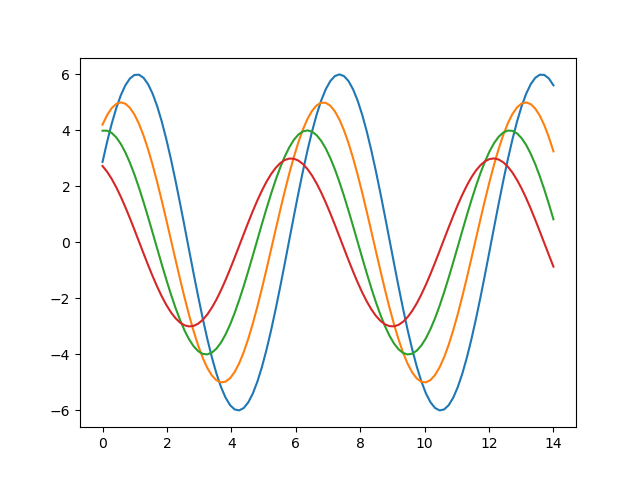
\includegraphics[width=0.8\textwidth]{gambar4_1}
    \label{fig:4_1}
\end{figure}

Untuk mengubah visual tersebut menjadi plot \textit{default} seaborn, kita dapat memanfaatkan fungsi \verb|set()|:
\lstinputlisting[language=Python]{contoh4_2.py}
Berikut ini luaran visual-nya:
\begin{figure}[H]
    \centering
    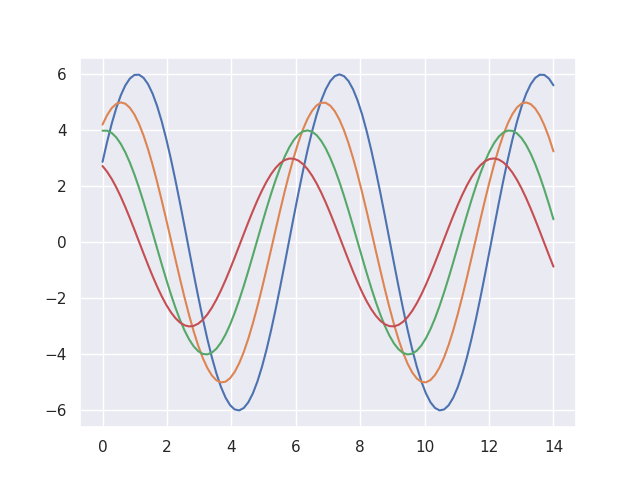
\includegraphics[width=0.8\textwidth]{gambar4_2}
    \label{fig:4_2}
\end{figure}

Dari kedua gambar tersebut, kita dapat memahami bahwa pada dasarnya representasi data yang dihasilkan oleh matplotlib dan seaborn bersifat identik, namun perbedaaan utamanya terletak pada estetika visualnya. Secara umum terdapat dua buah perbedaan antara seaborn dan matplotlib, yakni pada \textit{style} dan skala visualnya.

Untuk mengatur \textit{style} visual pada seaborn kita dapat memanfaatkan fungsi \verb|set_style()|. Dengan menggunakan fungsi ini kita dapat mengatur tema visual pada plot kita dengan lima tema berikut ini:
\begin{itemize}
    \item Darkgrid
    \item Whitegrid
    \item Dark
    \item White
    \item Ticks
\end{itemize}

Ok, sekarang waktunya kita mencoba mengubah tema pada plot kita menjadi whitegrid (karena \textit{default}-nya darkgrid):
\lstinputlisting[language=Python]{contoh4_3.py}
Berikut ini tampilannya:
\begin{figure}[H]
    \centering
    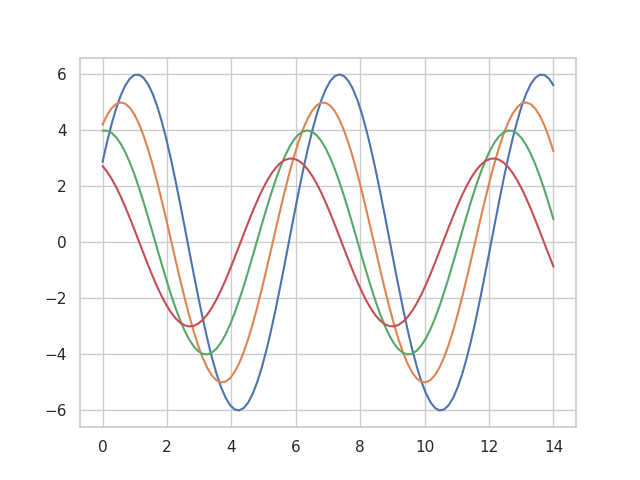
\includegraphics[width=0.8\textwidth]{gambar4_3}
    %\caption{Tahapan pengerjaan data}
    \label{fig:4_3}
\end{figure}
Yang menjadi perbedaan dibandingkan plot sebelumnya adalah tema latar belakangnya.

Pada tema white dan ticks, kita dapat membuang \textit{axis spine} pada sisi atas dan kanan plot dengan menggunakan fungsi \verb|despine()|:
\lstinputlisting[language=Python]{contoh4_4.py}

Berikut ini visualnya:
\begin{figure}[H]
    \centering
    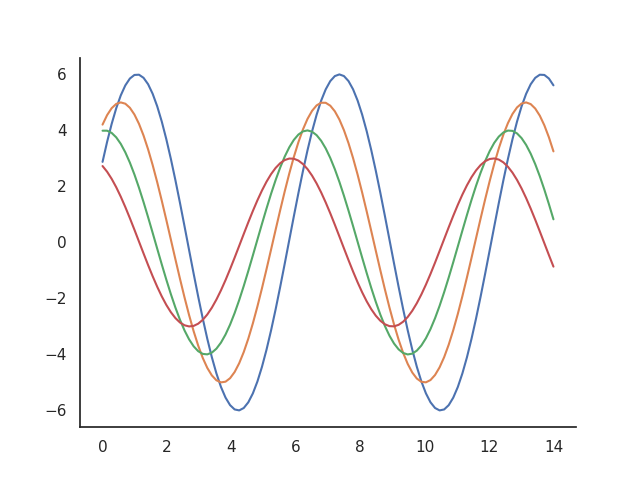
\includegraphics[width=0.8\textwidth]{gambar4_4}
    %\caption{Tahapan pengerjaan data}
    \label{fig:4_4}
\end{figure}

Jika kalian ingin mengkostumisasi \textit{style} pada tampilan seaborn kalian, kita dapat memasukkan \textit{dictionary} ke dalam fungsi \verb|set_style()|. Parameter - parameter yang dapat kita jadikan \textit{input}-an dapat dilihat menggunakan fungsi \verb|axes_style()|:
\lstinputlisting[language=Python]{contoh4_5.py}
Berikut ini luarannya:
\lstinputlisting[language={},numbers=none]{output4_5.txt}

Berikut ini salah satu contoh penerapannya:
\lstinputlisting[language=Python]{contoh4_6.py}
Yang akan menghasilkan visual seperti berikut ini:
\begin{figure}[H]
    \centering
    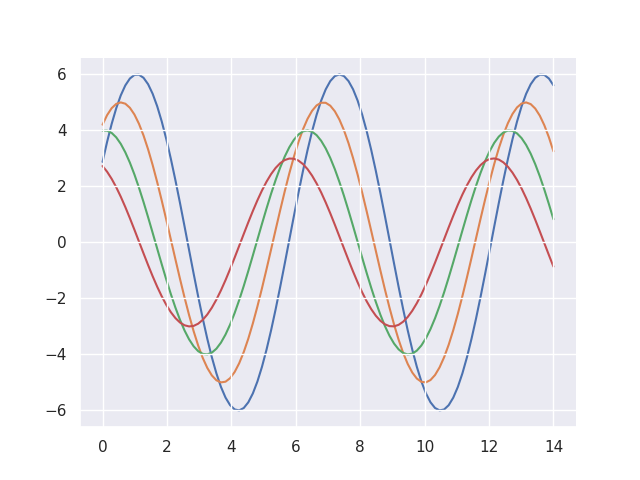
\includegraphics[width=0.8\textwidth]{gambar4_5}
    \label{fig:4_5}
\end{figure}

Di samping itu, seperti yang telah saya terangkan sebelumnya, kita juga dapat mengatur skala visual yang hendak kita hasilkan dengan menggunakan fungsi \verb|set.context()|. Pengaturan skala ini disesuaikan secara relatif terhadap konteks penggunaannya. Secara \textit{default} seaborn akan menyesuaikan dalam konteks notebook. Berikut ini konteks - konteks skala yang tersedia dalam pustaka seaborn:
\begin{itemize}
    \item Paper
    \item Notebook
    \item Talk
    \item Poster
\end{itemize}

Karena saya di sini menulisnya tidak pakai Jupyter notebook jadi tidak begitu terlihat perbedaan skalanya, namun coba \textit{deh} kalian jalankan program \href{https://github.com/sandyherho/buku_seaborn/blob/master/script/contoh4_7.py}{\textbf{ini}} nanti akan terlihat perbedaannya dibandingkan plot - plot sebelumnya:
\lstinputlisting[language=Python]{contoh4_7.py}

\textit{Punten} kalau perbedaan visual-nya tidak begitu terlihat, maklum \textit{scripting} \LaTeX{} dan Python -nya masih pakai vim hehe:
\begin{figure}[H]
    \centering
    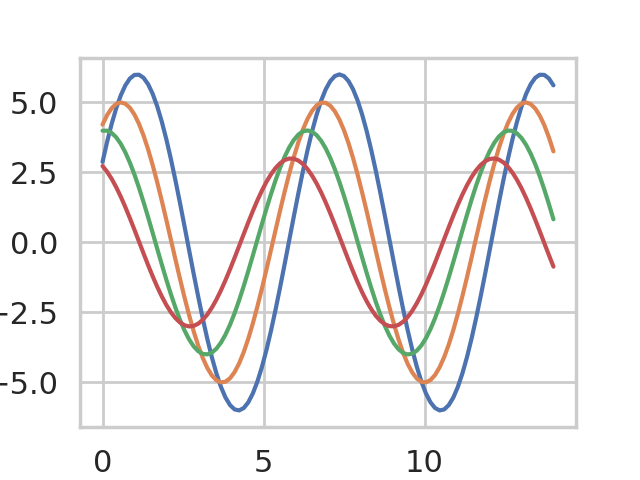
\includegraphics[width=1.0\textwidth]{gambar4_6}
    \label{fig:4_6}
\end{figure}

\chapter{Palet Warna}
Warna memainkan peranan paling penting dalam visualisasi data jika dibandingkan dengan aspek - aspek lainnya. Ketika kita menggunakan komposisi warna secara 'pas' maka plot kita akan tampak lebih bermakna dimata audiens, meskipun data yang kita hadirkan pada dasarnya sampah. Palet sendiri pada dasarnya bermakna sebagai suatu wadah tempat pelukis mencampurkan kombinasi warna. Hal yang mirip akan kita pelajari di bab ini, namun bentuknya tentu saja berbeda dengan palet para pelukis.

Untuk membuat palet warna, seaborn menyediakan fungsi \verb|color_palette()| yang dapat digunakan sebagai berikut ini:
\lstinputlisting[language=Python]{contoh5_1.py}
Pada tabel berikut ini, saya menampilkan parameter - parameter seaborn yang dibutuhkan untuk membentuk suatu palet warna:

\begin{table}[H]
\centering
\begin{tabularx}{\columnwidth}{|X|X|}
\hline\hline
\textbf{Jenis Parameter} & \textbf{Deskripsi} \\ [0.5ex]
\hline
\verb|palette| & Jenis palet yang hendak digunakan.\\
\verb|n_colors| & Jumlah warna dalam palet. Secara \textit{default} akan diisi dengan enam buah warna.\\
\verb|desat| & Proporsi desaturasi setiap warna.\\[1ex] 
\hline
\end{tabularx}
\end{table}

Berikut ini jenis - jenis palet yang telah disediakan oleh seaborn:
\begin{itemize}
    \item Deep
    \item Muted
    \item Bright
    \item Pastel
    \item Dark
    \item Colorblind
\end{itemize}
Di samping itu, kita juga dapat membuat palet warna sesuai keinginan kita sendiri.

Akan sangat sulit bagi kita untuk menentukan palet mana yang hendak kita pilih tanpa mengetahui karakteristik data yang hendak kita plot. Maka dari itu berhati-hatilah sebelum menentukan palet warna mana yang kalian pilih. Secara umum dapat diklasifikasikan tiga tipe data yang (mungkin) butuh palet warna yang berbeda, yakni:
\begin{itemize}
    \item kualitatif
    \item sekuensial
    \item kontras (\textit{diverging})
\end{itemize}

Untuk menampilkan palet - palet warna tersebut, seaborn mempunyai fungsi \verb|palplot()| yang ditujukkan untuk memvisualisasikan palet warna ke dalam bentuk \textit{array} horizontal.

Palet warna kualitatif seperti namanya, sangat cocok untuk memplot data yang bersifat kategoris. Berikut ini contoh visualnya:
\lstinputlisting[language=Python]{contoh5_2.py}
Hasilnya:
\begin{figure}[H]
    \centering
    
\includegraphics[width=0.8\textwidth]{gambar5_1}
    \label{fig:5_1}
\end{figure}

Kita belum memasukkan parameter apapun ke dalam fungsi \verb|color_palette()|, maka kita hanya dapat melihat enam buah warna yang terplot secara \textit{default}. Kita dapat mengubahnya dengan memasukkan jumlah warna yang kita kehendaki ke dalam parameter \verb|n_colors()|. Secara \textit{default} pula, fungsi \verb|palplot()| akan memplot \textit{array} palet warna secara horizontal.

Palet sekuensial sendiri bermanfaat untuk memvisualisasikan data yang membentang dari nilai paling rendah ke nilai paling tinggi. Kita harus menambahkan karakter \verb|s| sebagai masukkan warna dalam fungsi \verb|color_palette()| guna memplot palet sekuensial ini:
\lstinputlisting[language=Python]{contoh5_3.py}
Hasilnya:
\begin{figure}[H]
    \centering
    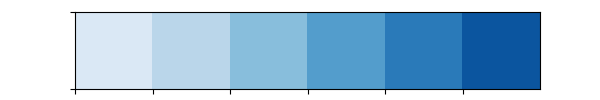
\includegraphics[width=0.8\textwidth]{gambar5_2}
    \label{fig:5_2}
\end{figure}

Jenis palet terakhir adalah palet kontras (\textit{diverging}) yang utamanya tersusun dari dua kutub warna yang berlainan dengan asumsi masing - masing kutub bernilai -1 dan +1 dengan titik pusat secara \textit{default} bernilai nol:
\lstinputlisting[language=Python]{contoh5_4.py}
Berikut ini visualnya:
\begin{figure}[H]
    \centering
    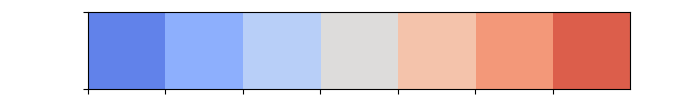
\includegraphics[width=0.8\textwidth]{gambar5_3}
    \label{fig:5_3}
\end{figure}

Terdapat juga fungsi lain yang mempunyai banyak kemiripan dengan fungsi \verb|color_palette()|, yakni fungsi \verb|set_palette()|. Berikut ini contoh penggunaannya:
\lstinputlisting[language=Python]{contoh5_5.py}
Hasilnya:
\begin{figure}[H]
    \centering
    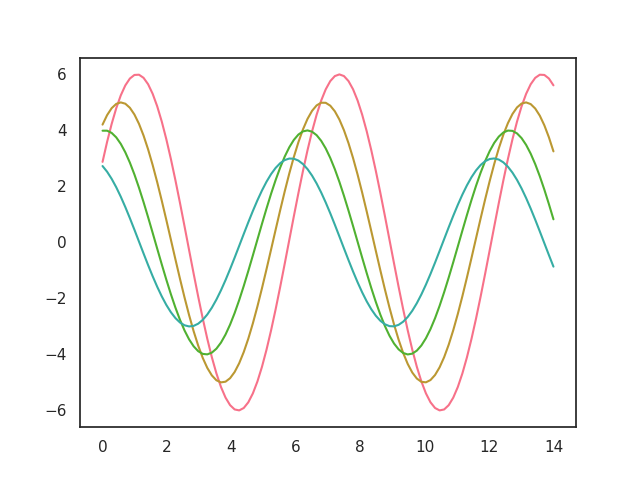
\includegraphics[width=0.8\textwidth]{gambar5_4}
    \label{fig:5_4}
\end{figure}

\chapter{Visualisasi Distribusi Univariat}
Distribusi dari suatu data merupakan hal pokok yang wajib diketahui oleh para analis ketika pertama kali dihadapkan pada data. Pada bab ini kita akan melihat bagaimana seaborn akan mempermudah kita dalam menganalisis distribusi data univariat.

Kita akan memanfaatkan fungsi \verb|distplot()| guna memvisualisasikan distribusi data univariat. Fungsi ini akan memvisualisasikan histogram yang sesuai dengan estimasi kepadatan kernel/\textit{Kernel Density Estimation} (KDE) dari data. Berikut ini bentuk umum dari fungsi ini:
\begin{verbatim}
    sns.distplot()
\end{verbatim}
Dengan parameter - parameter sebagai berikut:
\begin{table}[H]
\centering
\begin{tabularx}{\columnwidth}{|X|X|}
\hline\hline
\textbf{Parameter} & \textbf{Jenis Data} \\ [0.5ex]
\hline
\verb|data| & Jenis data yang dapat dijadikan masukkan antara lain adalah \textit{Series}, \textit{array} 1D, dan \textit{list}\\
\verb|bins| & Jumlah batang dalam histogram.\\
\verb|hist| & Berbentuk \textit{boolean}\\
\verb|kde| & Berbentuk \textit{boolean}.\\[1ex] 
\hline
\end{tabularx}
\end{table}

\section{Histogram}
Histogram merupakan visualisasi grafis distrbusi data dalam bentuk batang yang membentang di sepanjang rentang data. 

Seperti yang telah saya terangkan pada bab - bab awal, seaborn dilengkapi dengan beberapa dataset bawaan yang dapat kita manfaatkan sebagai medan berlatih. Pada bab ini kita akan menggunakan dataset \verb|iris|. Berikut ini \href{https://github.com/sandyherho/buku_seaborn/blob/master/script/contoh6_1.py}{program} untuk menunjukkan histogram panjang kelopak bunga iris (\verb|petal_length|):
\lstinputlisting[language=Python]{contoh6_1.py}
Berikut ini tampilan histogram-nya:
\begin{figure}[H]
    \centering
    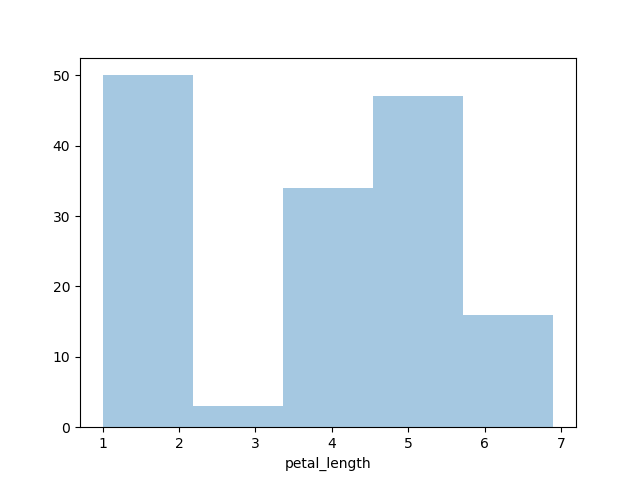
\includegraphics[width=0.8\textwidth]{gambar6_1}
    \label{fig:6_1}
\end{figure}

Pada contoh tersebut, saya mengatur parameter \verb|kde=False|, sehingga grafik tersebut tidak menampilkan KDE, hanya histogram saja yang ditampilkan.

\section{Estimasi Kepadatan Kernel (KDE)}
KDE merupakan salah satu cara untuk menghitung fungsi kepadatan peluang dari suatu peubah acak yang bersifat kontinyu. KDE digunakan untuk analisis non-parametrik. Untuk memvisualisasikan KDE dengan fungsi \verb|distplot()|, kita harus mengatur parameter \verb|hist=False| seperti pada contoh berikut \href{https://github.com/sandyherho/buku_seaborn/blob/master/script/contoh6_2.py}{ini}:
\lstinputlisting[language=Python]{contoh6_2.py}
Berikut ini visual-nya:
\begin{figure}[H]
    \centering
    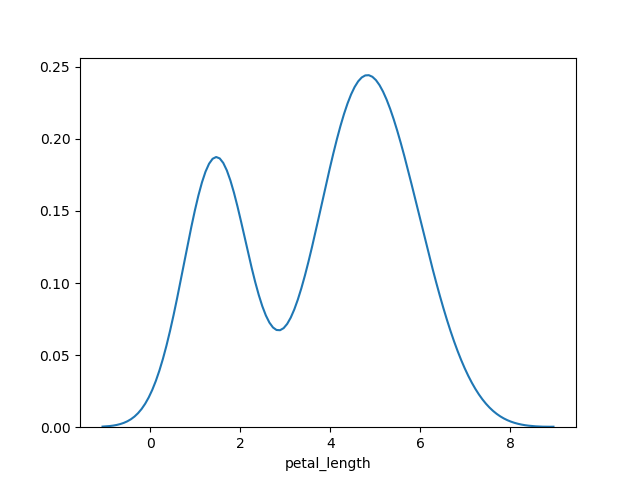
\includegraphics[width=0.8\textwidth]{gambar6_2}
    \label{fig:6_2}
\end{figure}

\section{Grafik KDE-Histogram}
Kita juga dapat menggabungkan kedua grafik distribusi univariat ini:
\lstinputlisting[language=Python]{contoh6_3.py}
\begin{figure}[H]
    \centering
    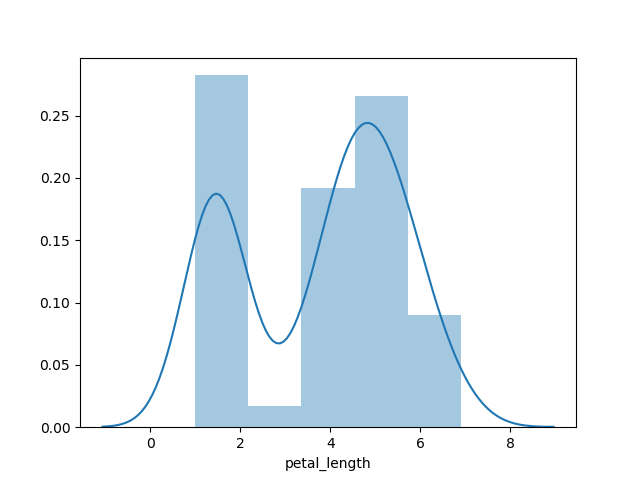
\includegraphics[width=0.8\textwidth]{gambar6_3}
    \label{fig:6_3}
\end{figure}

\chapter{Visualisasi Distribusi Bivariat}
Distribusi bivariat digunakan untuk menentukan hubungan antar dua peubah. Cara terbaik untuk mengetahui hubungan antara dua peubah ini adalah dengan memvisualisasikan distribusinya dengan menggunakan fungsi \verb|jointplot()|. Fungsi ini dapat menggambarkan hubungan antar kedua peubah, sekaligus juga mengetahui distribusi univariat masing - masing peubah pada sumbu terpisah.

\section{\textit{Scatter Plot}}
\textit{Scatter plot} merupakan cara paling sederhana untuk memvisualisasikan distribusi data dua peubah yang masing - masing diwakili oleh sumbu-x dan sumbu-y:
\lstinputlisting[language=Python]{contoh7_1.py}
\begin{figure}[H]
    \centering
    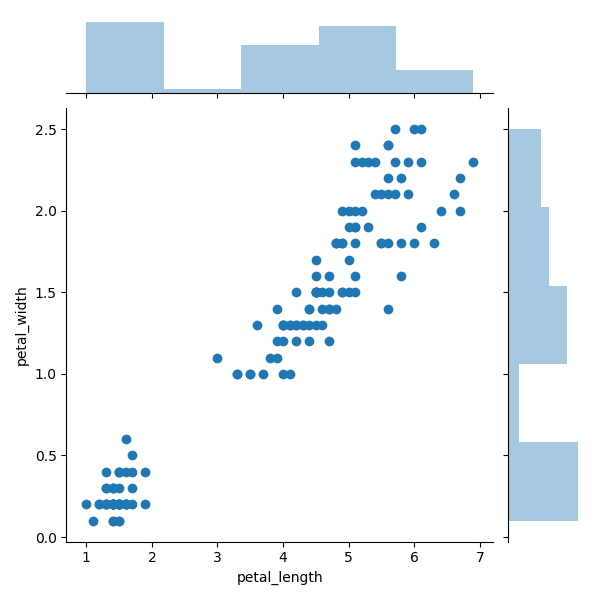
\includegraphics[width=0.8\textwidth]{gambar7_1}
    \label{fig:7_1}
\end{figure}
Gambar di atas menunjukkan hubungan antara peubah panjang dan lebar kelopak bunga iris. Nampak pada grafik hubungan berbanding lurus (korelasi positif) antar kedua peubah tersebut.

\section{Grafik \textit{Hexbin}}
Grafik heksagonal umumnya digunakan untuk menganalisis data bivariat yang sangat tersebar dan sukar dianalisis ketika divisualisasikan dengan \textit{scatter plot}. Untuk memvisualisasikan grafik ini, kita tinggal mengganti parameter \verb|kind='hex'| pada fungsi \verb|jointplot()|:
\lstinputlisting[language=Python]{contoh7_2.py}
\begin{figure}[H]
    \centering
    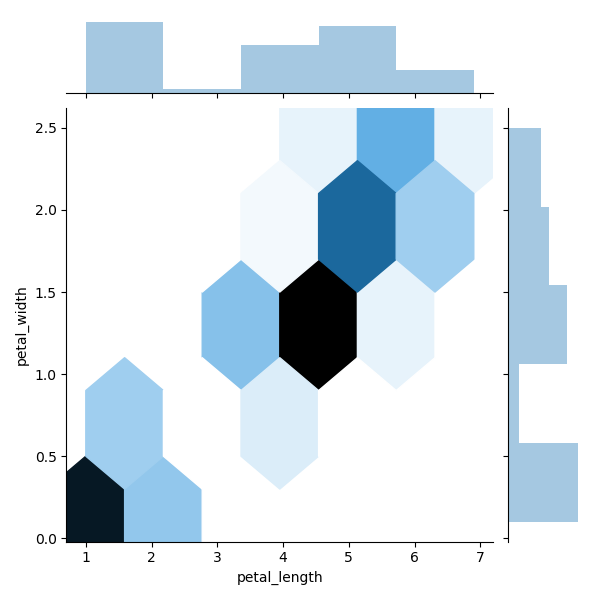
\includegraphics[width=0.8\textwidth]{gambar7_2}
    \label{fig:7_2}
\end{figure}
\section{Grafik KDE Bivariat}
Seperti yang saya jelaskan pada bab sebelumnya, KDE merupakan salah satu cara non-parametrik untuk mengestimasikan distribusi suatu peubah. Untuk distribusi bivariat, kita juga dapat memvisualisasikan grafik KDE dengan memasukkan parameter \verb|kind='kde'|. Perhatikanlah contoh berikut ini:
\lstinputlisting[language=Python]{contoh7_3.py}
\begin{figure}[H]
    \centering
    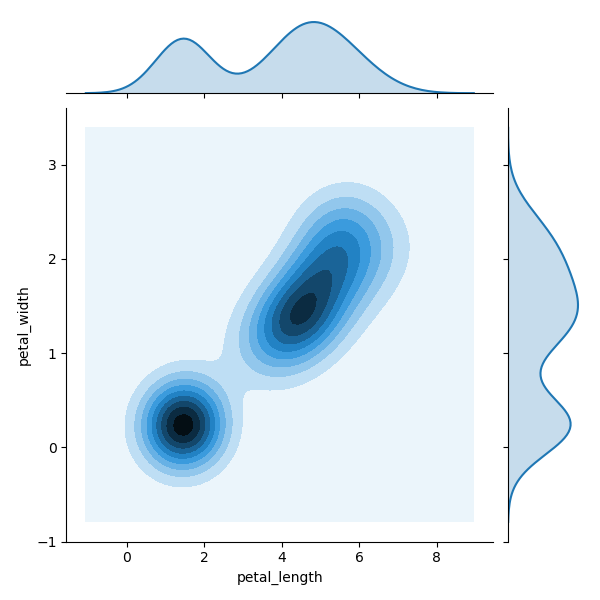
\includegraphics[width=0.8\textwidth]{gambar7_3}
    \label{fig:7_3}
\end{figure}

\chapter{Visualisasi Hubungan Antar Banyak Peubah}
Dalam penelitian yang sebenarnya, kita kerap kali dihadapkan dengan data yang mempunyai banyak peubah. Dalam kasus ini, tentunya kita harus menganalisis hubungan antar peubah secara keseluruhan. Namun, tentu kita berpikir akan sangat sulit dan memakan banyak waktu untuk memvisualisasikan distribusi bivariat untuk setiap kombinasi (n,2) pada masing - masing peubah. Untungnya dalam pustaka seaborn, kita dimudahkan dengan terdapatnya fungsi \verb|pairplot()|. Fungsi ini dapat menggambarkan grafik kombinasi (n,2) dari setiap peubah data dalam bentuk matriks, dengan diagonal utamanya merupakan representasi grafis dari data univariat. Berikut ini bentuk umum penggunaan fungsi \verb|pairplot()|:
\begin{verbatim}
    sns.pairplot(data,...)
\end{verbatim}

Parameter - parameter yang diperhitungkan adalah sebagai berikut:

\begin{table}[H]
\centering
\begin{tabularx}{\columnwidth}{|X|X|}
\hline\hline
\textbf{Jenis Parameter} & \textbf{Deskripsi} \\ [0.5ex]
\hline
\verb|data| & Berbentuk \textit{Data Frame}.\\
\verb|hue| & Pembedaan warna untuk aspek - aspek tertentu dalam data\\
\verb|palette| & Himpunan warna yang digunakan untuk pemetaan parameter \verb|hue|.\\
\verb|kind| & Jenis visualisasi data untuk peubah yang tidak identik, misalnya \verb|{'scatter', 'reg'}.|\\
\verb|diag_kind| & Jenis visualisasi data untuk visualisasi univariat pada diagonal utama dalam bentuk \verb|{'hist', 'kde'}|.\\[1ex] 
\hline
\end{tabularx}
\end{table}

Selain parameter data, parameter - parameter lainnya bersifat opsional. Selain parameter - parameter tersebut, sesungguhnya fungsi \verb|pairplot()| masih dapat menerima masukkan parameter - parameter lainnya yang tidak akan dibahas dalam tutorial ini karena tidak lazim digunakan dalam analisis konvensional. Berikut ini contoh penerapan \verb|pairplot()|:
\lstdefinestyle{language=Python}{contoh8_1.py}
\begin{figure}[H]
    \centering
    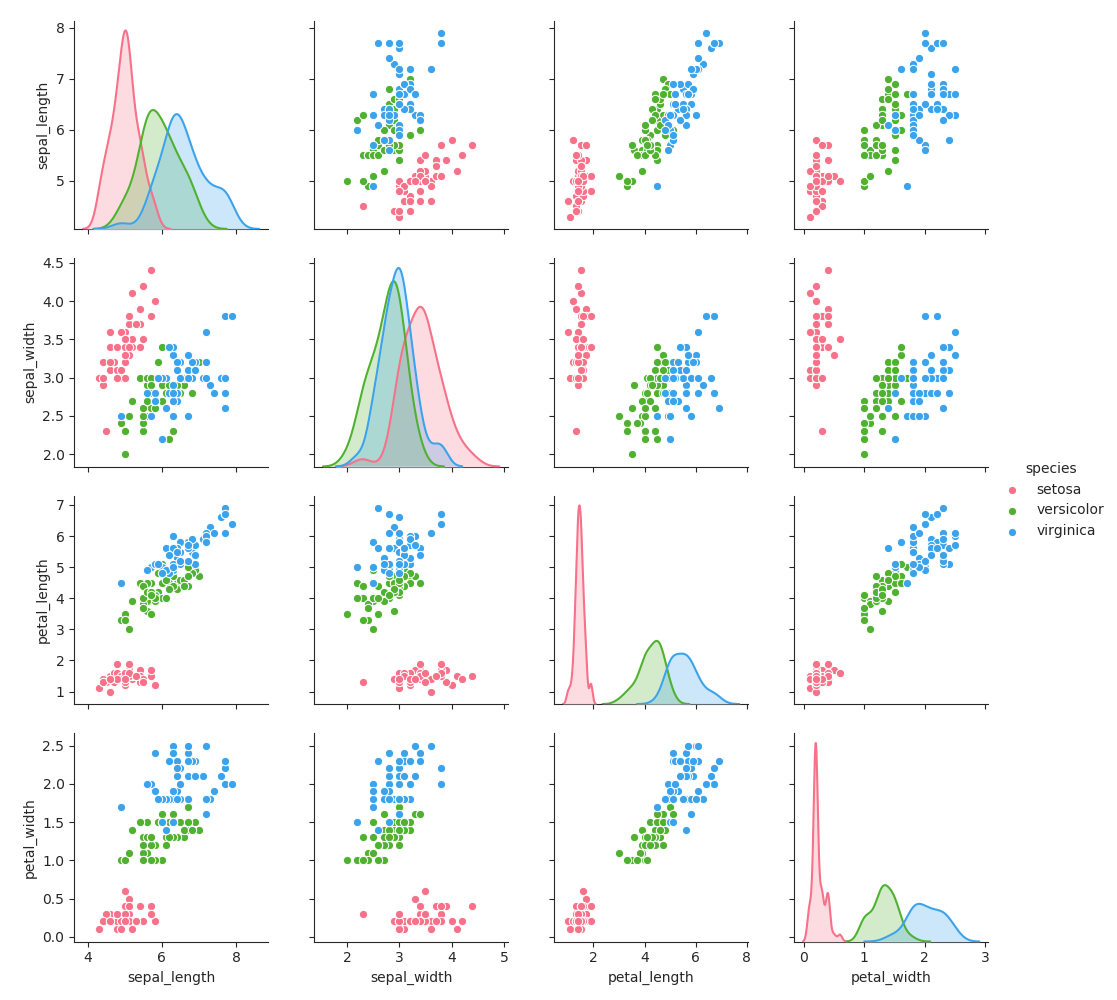
\includegraphics[width=1.0\textwidth]{gambar8_1}
    \label{fig:8_1}
\end{figure}
Melalui diagram tersebut kita dapat menganalisis perubahan hubungan bivariat pada masing - masing peubah.

\chapter{Visualisasi Data Kategoris}
Pada bagian sebelumnya kita telah mempelajari tentang \textit{scatter plot}, grafik \textit{hexbin}, dan grafik KDE. Grafik - grafik tersebut ditujukkan untuk memvisualisasikan data yang bersifat kontinyu, namun tidak dapat digunakan untuk visualisasi data yang bersifat kategoris. Pada bagian ini kita akan membahas fitur - fitur visualisasi data kategoris dengan menggunakan seaborn.
\section{\textit{Categorical Scatter Plots}}
Terdapat dua jenis \textit{scatter plot} yang dapat kita manfaatkan untuk memvisualisasikan data kategoris, yakni \verb|stripplot()| dan \verb|swarmplot()|.

Grafik \verb|stripplot()| digunakan untuk menjelaskan distribusi suatu data, jika salah satu dari peubahnya bersifat kategoris. Grafik ini merepresentasikan data yang diurutkan pada salah satu sumbu. Berikut ini contohnya:
\lstinputlisting[language=Python]{contoh9_1.py}
\begin{figure}[H]
    \centering
    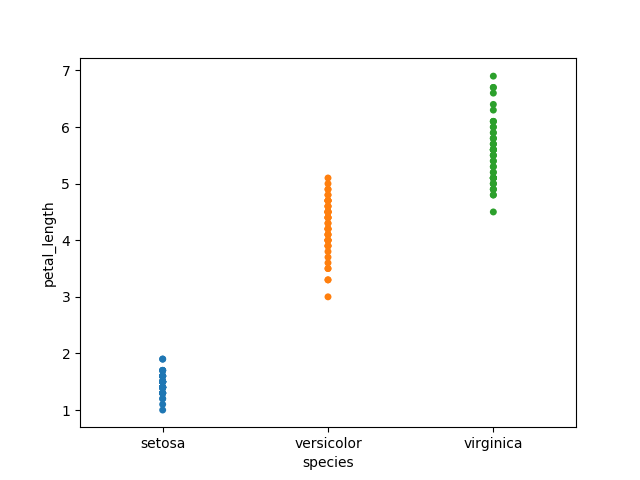
\includegraphics[width=1.0\textwidth]{gambar9_1}
    \label{fig:9_1}
\end{figure}
Pada grafik di atas kita dapat dengan jelas melihat perbedaan panjang kelopak bunga pada masing - masing spesies. Namun, salah satu permasalahan utama pada \textit{scatter plot} adalah bertumpuknya titik - titik data, sehingga distribusi data tidak terlihat secara jelas. Guna memperjelas distribusi data, kita umumnya menggunakan parameter \verb|jitter=True| untuk menambahkan \textit{random noise} pada data:
\lstinputlisting[language=Python]{contoh9_2.py}
\begin{figure}[H]
    \centering
    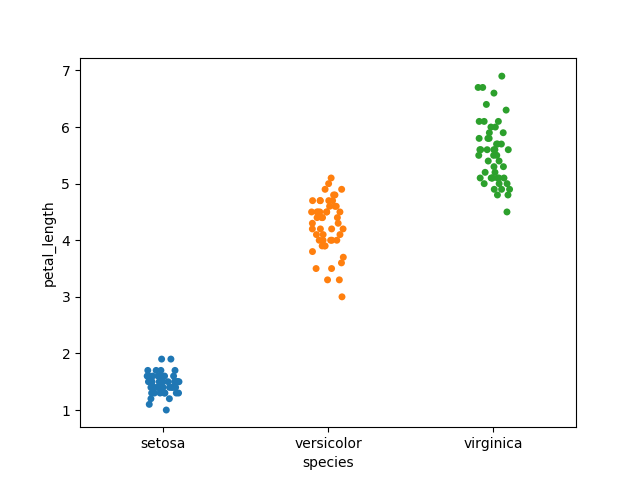
\includegraphics[width=1.0\textwidth]{gambar9_2}
    \label{fig:9_2}
\end{figure}

Salah satu opsi lain untuk menghindari titik - titik data yang bertumpuk adalah dengan menggunakan grafik \verb|swarmplot()|. Fungsi ini menempatkan setiap titik data dalam \textit{scatter plot} pada masing - masing sumbu kategoris, sehingga menghindari bertumpang tindihnya titik - titik data:
\lstinputlisting[language=Python]{contoh9_3.py}
\begin{figure}[H]
    \centering
    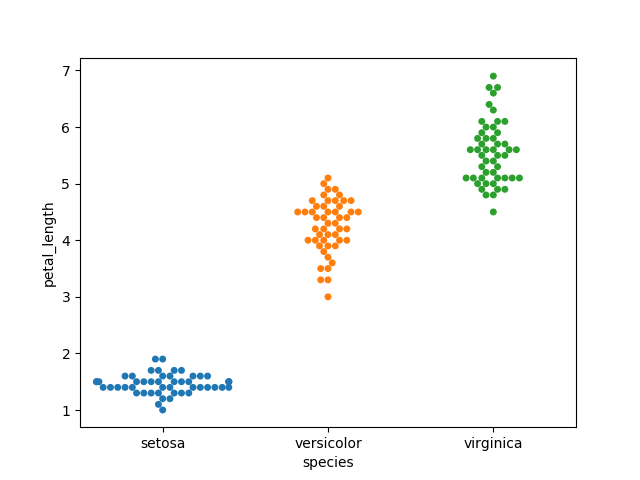
\includegraphics[width=1.0\textwidth]{gambar9_3}
    \label{fig:9_3}
\end{figure}

\section{Grafik - Grafik Untuk Mengetahui Perbandingan Data Kategoris}
Pada sub-bab sebelumnya kita telah melihat bagaimana perbandingan distribusional antar kategori - kategori data. Namun hal tersebut masih tampak kabur karena yang terlihat hanya persebaran data secara kualitatif. Pada bagian ini kita mencoba menggambarkan distribusi data secara lebih jelas dengan menggunakan \textit{box plot} dan \textit{violin plot}.
\subsection{\textit{Box Plot}}
\textit{Box plot} merupakan cara paling mudah untuk menggambarkan distribusi data kategoris sesuai dengan jangkauan kuartilnya. \textit{Box plot} mempunyai garis vertikal yang memanjang keluar dari kotak yang dikenal dengan istilah \textit{whisker}. \textit{Whisker} inilah yang menggambarkan variabilitas data di luar batas kuartil atas dan kuartil bawah (atau yang dikenal sebagai pencilan). Maka dari itu, terkadang \textit{box plot} juga dikenal sebagai diagram \textit{box-whisker}. Seluruh pencilan dalam \textit{box plot} divisualisasikan sebagai titik - titik individual di luar kotak. Berikut ini contoh penerapan \textit{box plot} dengan menggunakan seaborn:
\lstinputlisting[language=Python]{contoh9_4.py}
\begin{figure}[H]
    \centering
    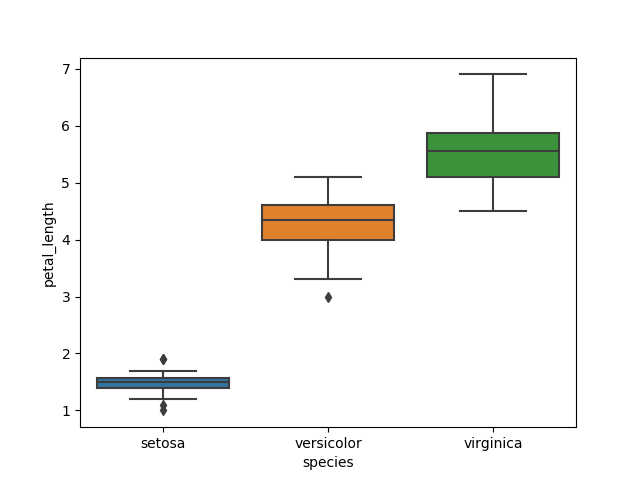
\includegraphics[width=1.0\textwidth]{gambar9_4}
    \label{fig:9_4}
\end{figure}
Titik - titik di bagian luar kotak mengindikasikan data pencilan.

\subsection{\textit{Violin Plot}}
\textit{Violin plot} merupakan kombinasi dari \textit{box plot} dan KDE, sehingga memudahkan para analis data untuk memahami distribusi data kontinyu pada masing - masing kategori. Untuk lebih memahami \textit{violin plot}, kita akan mempleajarinya dengan menggunakan data bawaan \verb|tips| pada seaborn:
\lstinputlisting[language=Python]{contoh9_5.py}
\begin{figure}[H]
    \centering
    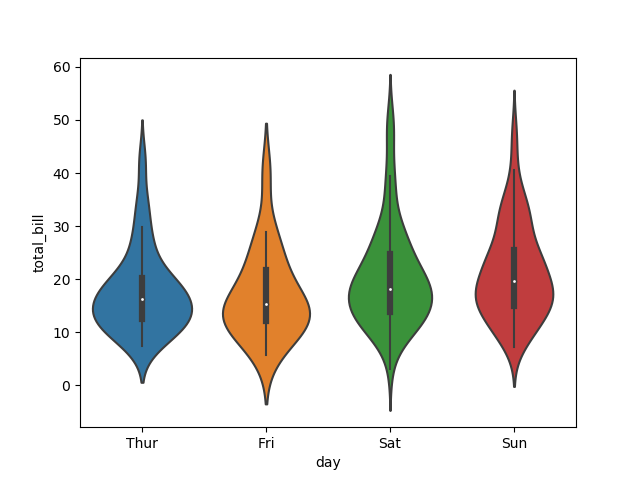
\includegraphics[width=1.0\textwidth]{gambar9_5}
    \label{fig:9_5}
\end{figure}

Pada \textit{violin plot}, nilai -nilai kuartil dan \textit{whisker} dimasukkan di dalam grafik. Oleh karena dalam perhitungannya \textit{violin plot} memasukkan fungsi KDE, maka bagian grafik yang tampak cembung mengindikasikan kepadatan peluang yang besar, pun berlaku sebaliknya pada bagian yang pipih mengindikasikan rendahnya nilai kepadatan peluang. Jangkauan antar kuartil pada \textit{box plot} berada pada wilayah yang sama dengan KDE berkepadatan tinggi pada \textit{violin plot}.

Grafik di atas menunjukkan distribusi total pembayaran pada empat hari dalam seminggu. Kita dapat melakukan eksplorasi data secara lebih mendalam pada grafik tersebut dengan memisahkan total pembayaran tip berdasarkan jenis kelamin, seperti pada contoh berikut ini:
\lstinputlisting[language=Python]{contoh9_6.py}
\begin{figure}[H]
    \centering
    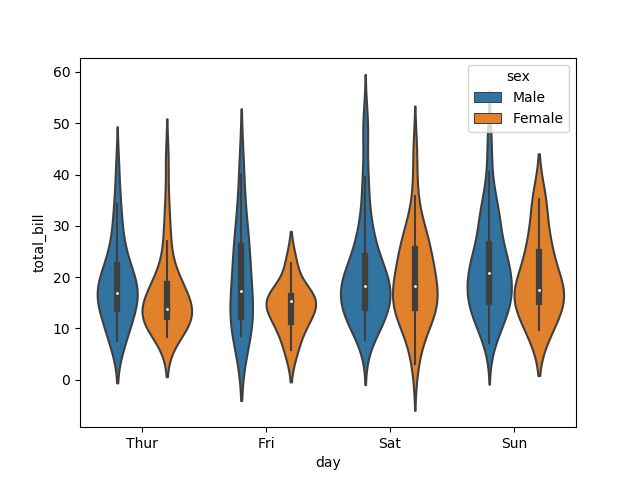
\includegraphics[width=1.0\textwidth]{gambar9_6}
    \label{fig:9_6}
\end{figure}

Sekarang kita sudah dapat meihat secara jelas distribusi pengeluaran per hari untuk tip berdasarkan jenis kelamin pelanggan. Bukan bermaksud anti-feminis, namun dari data 'bohongan' di atas terlihat bahwa pria menghabiskan lebih banyak uang untuk tip di restoran tersebut dibandingkan dengan wanita.

Karena \verb|hue| data ini hanya terdiri dari dua kategori, yakni pria dan wanita, maka untuk alasan estetika kita dapat membagi \textit{violin plot} menjadi dua bagian agar grafik-nya lebih 'enak' dipandang mata:
\lstinputlisting[language=Python]{contoh9_7.py}
\begin{figure}[H]
    \centering
    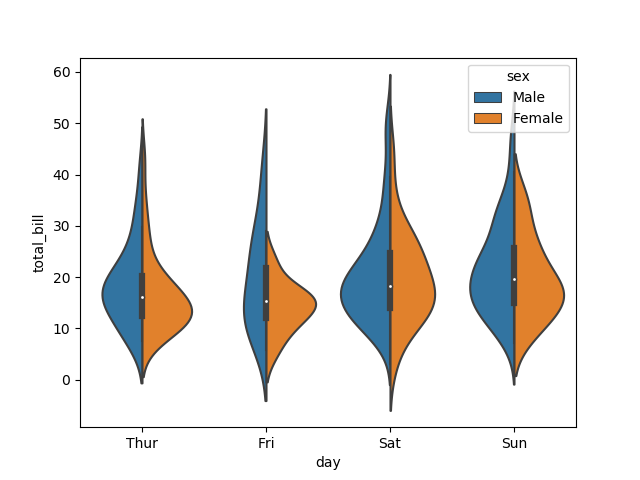
\includegraphics[width=1.0\textwidth]{gambar9_7}
    \label{fig:9_7}
\end{figure}

\chapter{Visualisasi Tendensi Sentral}
Dalam kebanyakan kasus penelitian, utamanya pada bidang klimatologi, kita harus berhadapan dengan estimasi seluruh distrbusi data. Namun terkadang dalam penelitian - penelitian tertentu, terkadang kita hanya perlu untuk merangkum estimasi sentral dari suatu data. Rata - rata dan median merupakan dua ukuran tendensi sentral yang selalu dikerjakan dalam segala jenis penelitian.

Pada bagian - bagian sebelumnya kita telah melakukan visualisasi untuk seluruh distribusi data, pada bagian ini kita akan membahas visualisasi yang berhubungan dengan estimasi tendensi sentral dari distribusi data secara statistik.

\section{Diagram Batang}
Diagram batang menunjukkan relasi antara peubah kategoris dan peubah kontinyu. Data disajikan dalam format persegi panjang, di mana panjang setiap batang merepresentasikan proporsi data pada masing - masing kategori. Melalui diagram batang kita dapat memperkirakan kisaran nilai tendensi sentral dari suatu data. Berikut ini contoh visualisasi diagram batang dengan menggunakan dataset \verb|titanic| pada seaborn:
\lstinputlisting[language=Python]{contoh10_1.py}
\begin{figure}[H]
    \centering
    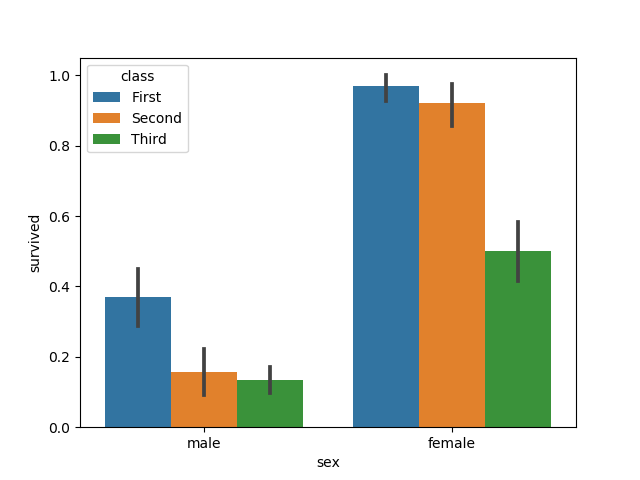
\includegraphics[width=1.0\textwidth]{gambar10_1}
    \label{fig:10_1}
\end{figure}

Melalui diagram di atas, kita dapat mengetahui rata - rata pria dan wanita yang selamat dalam kasus tenggelamnya kapal titanic pada masing - masing kelas. Nampak bahwa jumlah wanita yang selamat lebih banyak dari pria, dan jumlah penumpang yang selamat lebih tinggi pada kelas 1.

Untuk mengetahui jumlah eksak masing - masing kategori data, kita dapat menggunakan fungsi \verb|countplot()|:
\lstinputlisting[language=Python]{contoh10_2.py}
\begin{figure}[H]
    \centering
    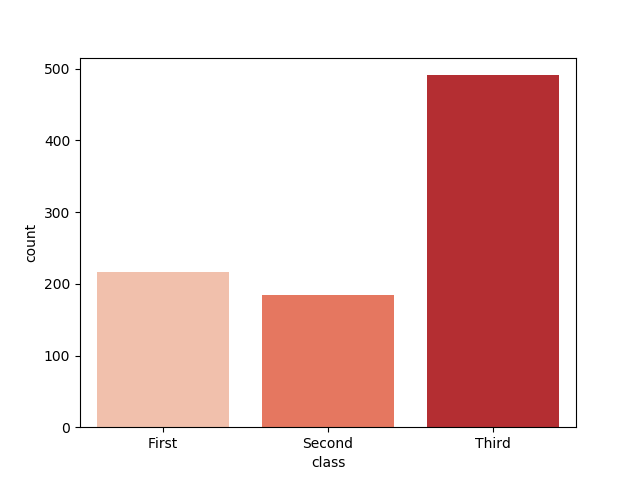
\includegraphics[width=1.0\textwidth]{gambar10_2}
    \label{fig:10_2}
\end{figure}

\section{Diagram Titik}
Diagram titik pada dasarnya mempunyai banyak kemiripan dengan diagram batang, hanya gaya visualisasinya saja yang berbeda, yakni dengan merepresentasikan sebaran data pada titik dengan ketinggian tertentu. Perhatikanlah contoh berikut ini:
\lstinputlisting[language=Python]{contoh10_3.py}
\begin{figure}[H]
    \centering
    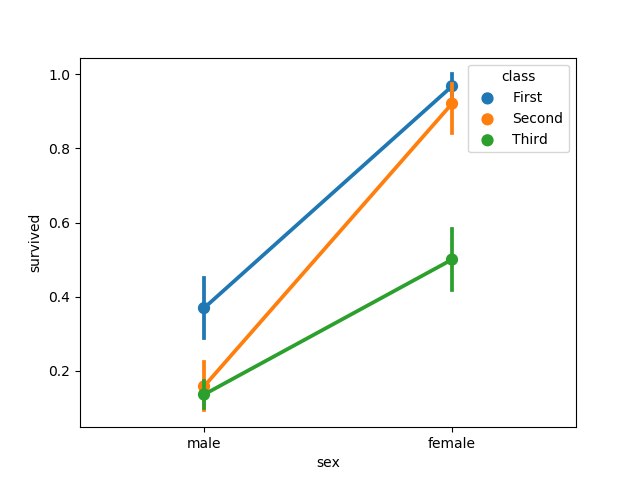
\includegraphics[width=1.0\textwidth]{gambar10_3}
    \label{fig:10_3}
\end{figure}

\chapter{Visualisasi Data Berformat Melebar}

Umumnya sebagai analis data kita mengharapkan data yang hendak kita olah berformat memanjang dengan sedikit nilai kosong, namun terkadang kita dihadapkan pada data yang berformat melebar, sehingga mau tidak mau kita harus melakukan pengolahan tanpa melakukan pengubahan dimensi (\verb|reshape()|) karena dikhawatirkan dapat mengubah makna fisis dari data tersebut. Untuk menangani visualisasi data tersebut, kita hanya tinggal mengubah parameter orientasi pada grafik seaborn yang hendak kita plot seperti pada dua contoh berikut ini:
\lstinputlisting[language=Python]{contoh11_1.py}
\begin{figure}[H]
    \centering
    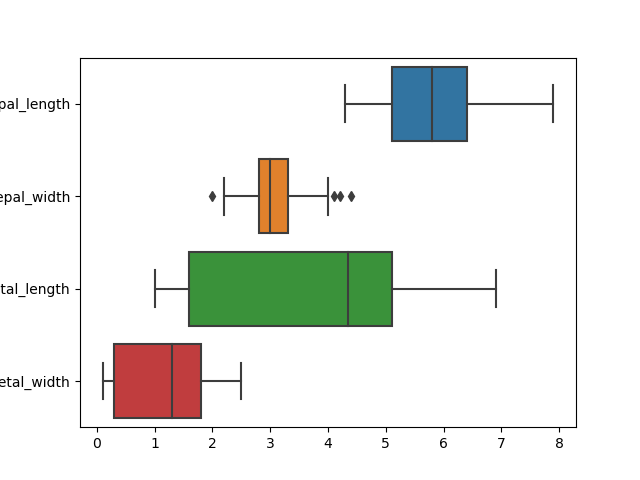
\includegraphics[width=0.8\textwidth]{gambar11_1}
    \label{fig:11_1}
\end{figure}

\lstinputlisting[language=Python]{contoh11_2.py}

\begin{figure}[H]
    \centering
    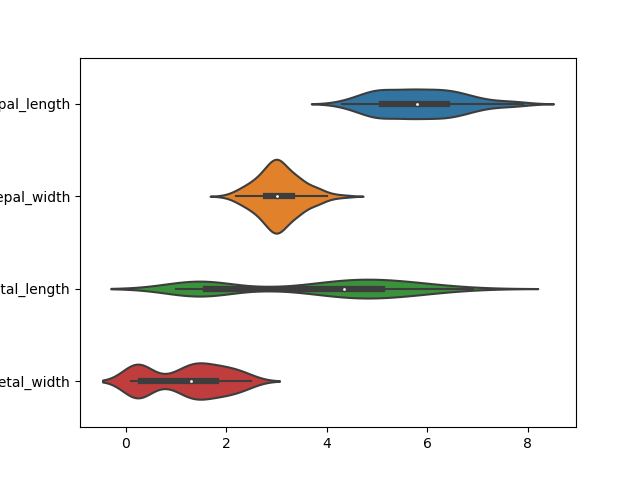
\includegraphics[width=0.8\textwidth]{gambar11_2}
    \label{fig:11_2}
\end{figure}
\chapter{Visualisasi Multi-Panel}
Salah satu pendekatan yang berguna untuk mendapatkan intisari dari suatu data berdimensi sedang adalah dengan cara memvisualisasikan masing - masing peubah pada kanvas yang sama, sehingga memungkinkan kita sebagai analis untuk menarik kesimpulan lebih mendalam. Bagian ini akan menampilkan dua bentuk visualisasi multi panel, yakni \textit{Facet Grid} dan \textit{Pair Grid}
\section{\textit{Facet Grid}}
\textit{Facet grid} digunakan untuk memvisualisasikan panel grafik berbentuk matriks, di mana setiap kolom dan baris merepresentasikan peubah data. Grafik ini sangat membantu ketika kita hendak menganalisis dua peubah diskrit.

Secara umum \textit{facet grid} tersusun dari tiga dimensi, yakni baris, kolom, dan \textit{hue}. Baris dan kolom berkorespondensi langsung terhadap sumbu data dalam grafik, sementara \textit{hue} dapat dikatakan sebagai sumbu 'z' dari data yang merepresentasikan peubah tertentu. \textit{Facet grid} hanya menerima data bertipe \textit{data frame} sebagai masukan, dan menjadikan nama dari peubah terpilih sebagai judul baris, kolom, dan \textit{hue}. Perlu kalian ingat, bahwa setiap peubah yang dijadikan masukan dalam \textit{facet grid} harus bersifat kategoris. Perhatikanlah contoh berikut ini:
\lstinputlisting[language=Python]{contoh12_1.py}
\begin{figure}[H]
    \centering
    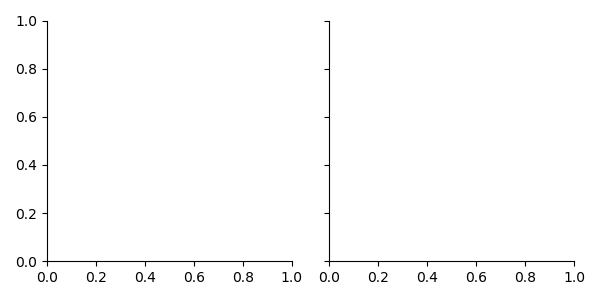
\includegraphics[width=1\textwidth]{gambar12_1}
    \label{fig:12_1}
\end{figure}

Pada contoh di atas, kita telah menginisialisasi objek \textit{facet grid} kosong pada kanvas. Untuk memvisualisasikan data pada kanvas tersebut umumnya para analis data menggunakan metode \verb|FacetGrid.map()| guna memetakan peubah yang hendak divisualisasikan dalam kanvas kosong tersebut. Dalam kasus ini, kita akan mencoba melihat distribusi tip yang diberikan berdasarkan waktu makan:
\lstinputlisting[language=Python]{contoh12_2.py}
\begin{figure}[H]
    \centering
    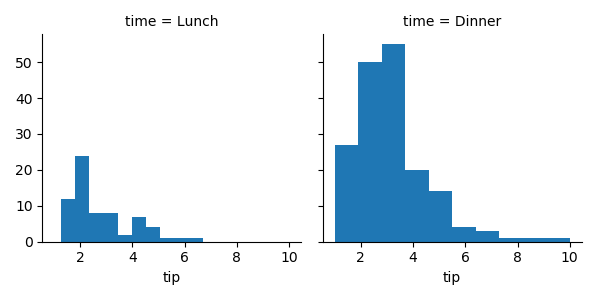
\includegraphics[width=1\textwidth]{gambar12_2}
    \label{fig:12_2}
\end{figure}

Jumlah plot-nya lebih dari satu karena ita masukkan parameter \verb|col| dengan peubah waktu makan. Berikut ini contoh visual penggunaan \textit{facet grid} dengan masukan banyak peubah:
\lstinputlisting[language=Python]{contoh12_3.py}
\begin{figure}[H]
    \centering
    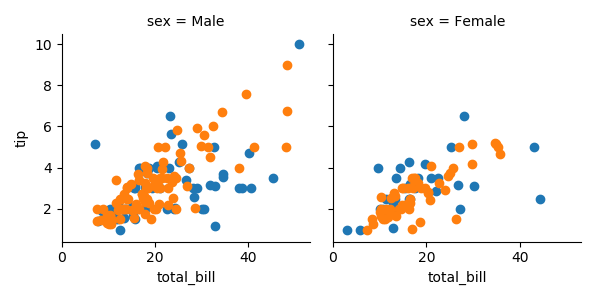
\includegraphics[width=1\textwidth]{gambar12_3}
    \label{fig:12_3}
\end{figure}

\section{\textit{Pair Grid}}
\textit{Pair grid} memungkinkan kita untuk menggunakan jenis visualisasi yang sama untuk setiap grid dalam sub-plot. Namun tidak sperti \textit{facet grid}, \textit{pair grid} menggunakan peubah yang berbeda untuk setiap peubah yang digunakan dalam sub-plot-nya. \textit{Pair grid} secara visual akan membentuk apa yang dinamakan sebagai matriks \textit{scatter plot}. Cara pengunaan \textit{pair grid} mirip dengan \textit{facet grid}, yakni diawali dengan inisialisasi objek dalam kanvas, kemudian menggunakan metode \verb|map()| untuk memetakan peubah yang hendak kita plot ke dalam objek kosong dalam kanvas. Berikut ini contoh penggunaannya:
\lstinputlisting[language=Python]{contoh12_4.py}
\begin{figure}[H]
    \centering
    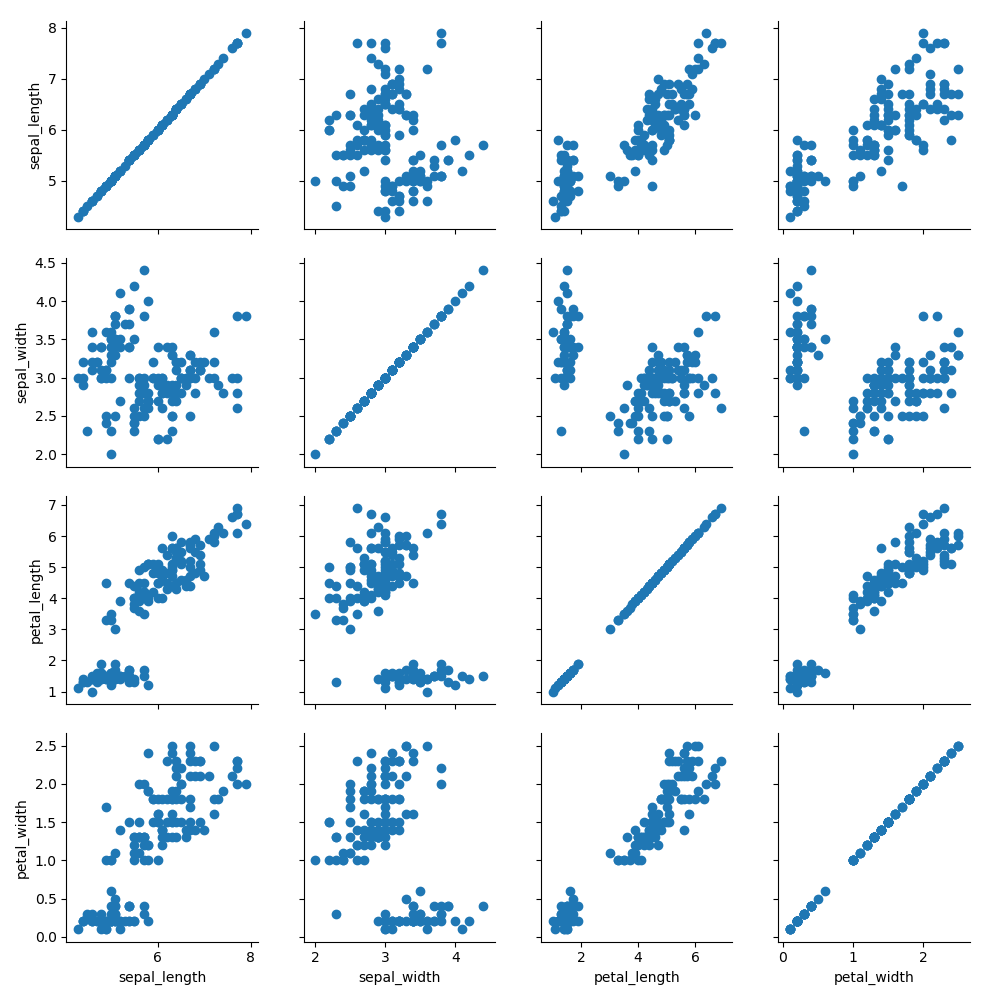
\includegraphics[width=1\textwidth]{gambar12_4}
    \label{fig:12_4}
\end{figure}

Selain itu, kita juga dapat mengubah tipe visualisasi pada diagonal matriks-nya, seperti dalam contoh ini saya menunjukkan distribusi univariat pada diagonal-nya:
\lstinputlisting[language=Python]{contoh12_5.py}
\begin{figure}[H]
    \centering
    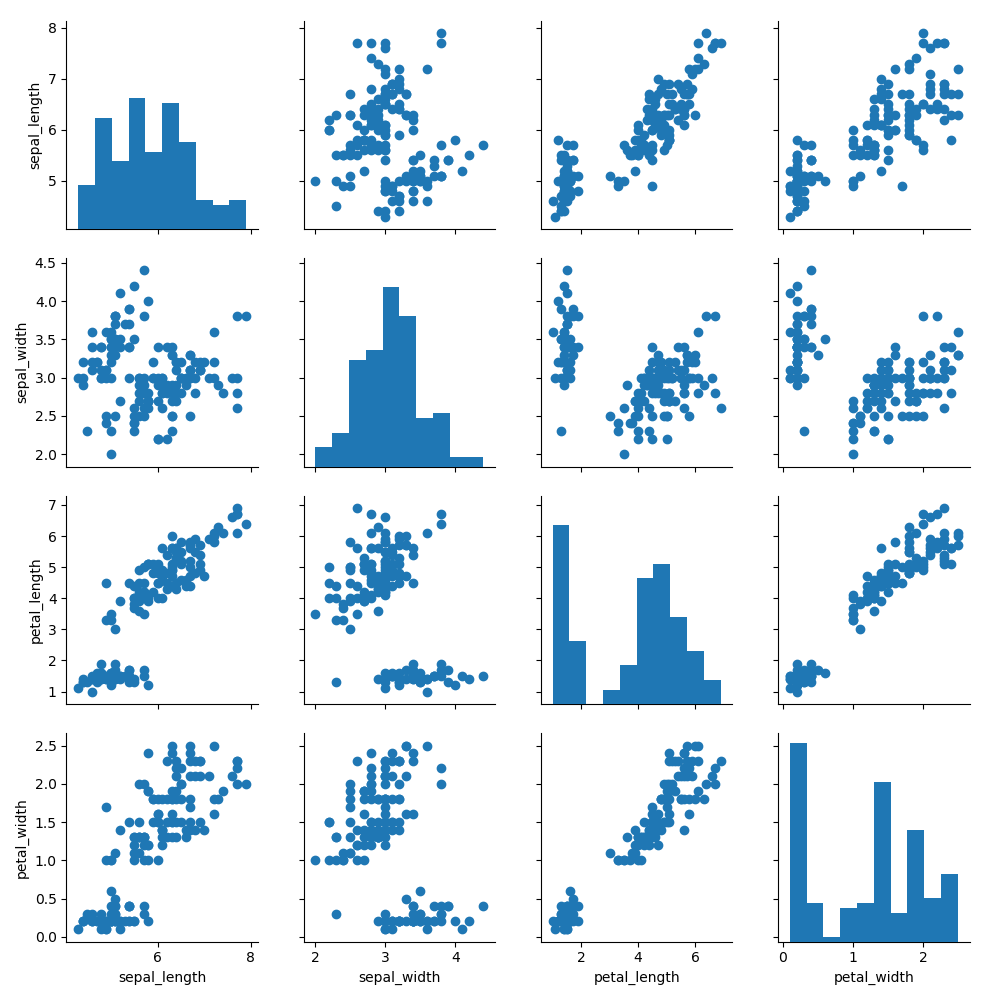
\includegraphics[width=1\textwidth]{gambar12_5}
    \label{fig:12_5}
\end{figure}
Kita juga dapat mengubah segitiga atas dan segitiga bawah pada matriks dengan tipe visualisasi yang berbeda:
\lstinputlisting[language=Python]{contoh12_6.py}
\begin{figure}[H]
    \centering
    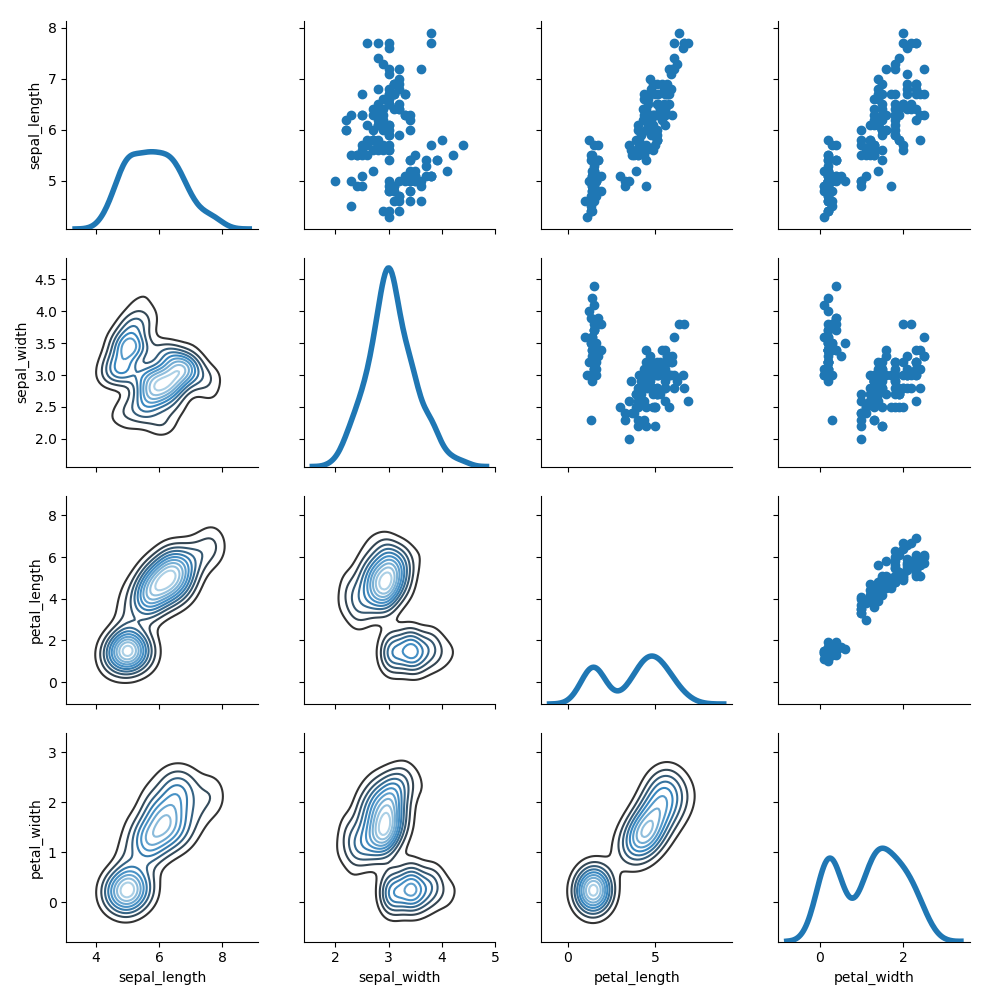
\includegraphics[width=1\textwidth]{gambar12_6}
    \label{fig:12_6}
\end{figure}
\chapter{Visualisasi Regresi Linier}
Kerap kali sebagai analis data kita diminta untuk menganalisis hubungan kuantitatif antar dua peubah. Untuk memenuhi hal ini, kita dapat melakukannya dengan visualisasi melalui metode regresi. Dengan menerapkan model regresi ini, kita dapat memeriksa multikolinieritas antar peubah yang hendak kita cari hubungannya. Bab ini akan membahas tentang visualisasi melalui model regresi dengan menggunakan seaborn.
\section{Fungsi - Fungsi Untuk Memvisualisasikan Regresi Linier}
Terdapat dua buah fungsi dalam seaborn yang dapat kita manfaatkan untuk memvisualisasikan regresi linier, yakni \verb|regplot()| dan \verb|lmplot()|, berikut ini perbedaan antar keduanya:
\begin{table}[H]
\centering
\begin{tabularx}{\columnwidth}{|X|X|}
\hline
\verb|regplot()| & Menerima berbagai jenis data masukkan, seperti \textit{array} numpy sederhana, \textit{series}, hingga \textit{data frame}. Hanya dapat memvisualisasikan regresi linier.\\ 
\verb|lmplot()| & Umumnya bekerja dengan lebih baik pada data berformat panjang (\textit{long-form format}). Dapat memproses regresi polinomial.\\[1ex] 
\hline
\end{tabularx}
\end{table}

Untuk melihat perbedaannya secara visual, perhatikanlah contoh berikut ini:
\lstinputlisting[language=Python]{contoh13_1.py}
\begin{figure}[H]
    \centering
    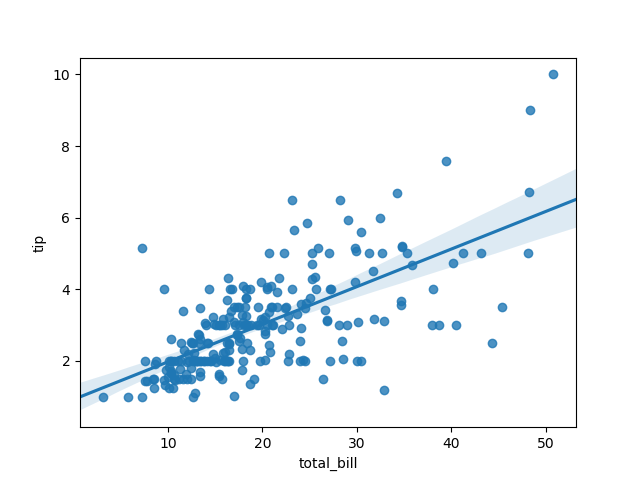
\includegraphics[width=1\textwidth]{gambar13_1a}
    \label{fig:13_1a}
    \captionsetup{labelformat=empty}
    \caption{Regresi Linier dengan fungsi regplot()}
\end{figure}
\begin{figure}[H]
    \centering
    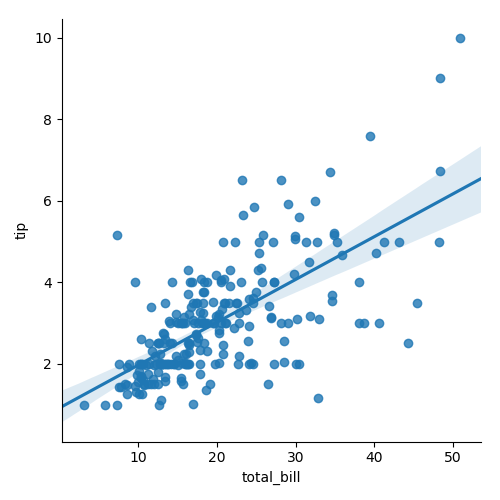
\includegraphics[width=1\textwidth]{gambar13_1b}
     \captionsetup{labelformat=empty}
    \caption{Regresi Linier dengan fungsi lmplot()}
    \label{fig:13_1b}
\end{figure}

Kedua grafik tersebut tampak identik, hanya saja terdapat perbedaan dari segi ukuran saja. Jadi kesimpulannya untuk visualisasi regresi linier, kita dapat memilih untuk menggunakan \verb|regplot()| atau \verb|lmplot()| sesuai kehendak kita.

Kita juga dapat melakukan pemodelan regresi linier pada dua peubah, di mana salah satu peubahnya bersifat diskrit:
\lstinputlisting[language=Python]{contoh13_2.py}
\begin{figure}[H]
    \centering
    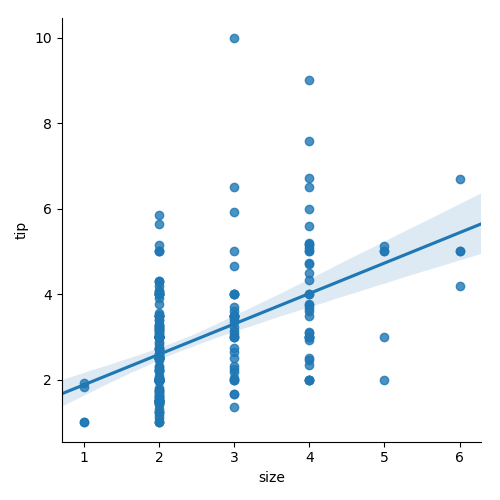
\includegraphics[width=1\textwidth]{gambar13_2}
    \label{fig:13_2}
\end{figure}

\section{\textit{Fitting} Model Non-linier}
Model regresi linier tidak selalu cocok untuk diterapkan pada semua kasus. Terkadang kita sebagai analis data harus memikirkan pendekatan non-linier ketika dihadapkan dengan kasus semacam ini. Perhatikanlah contoh - contoh pengolahan data \verb|anscombe| berikut ini:
\lstinputlisting[language=Python]{contoh13_3.py}
\begin{figure}[H]
    \centering
    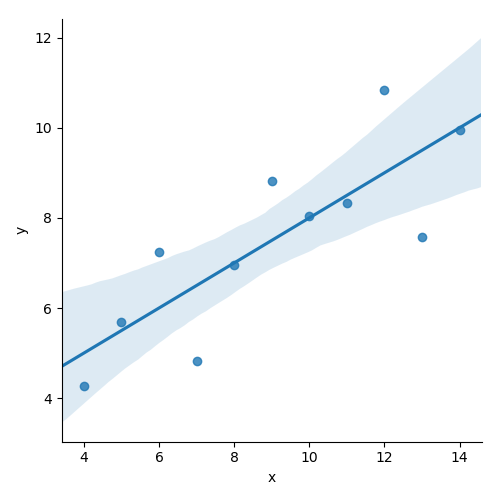
\includegraphics[width=1\textwidth]{gambar13_3}
    \label{fig:13_3}
\end{figure}
Pada kasus ini, kita beruntung karena model regresi linier cocok untuk diterapkan pada data ini dengan nilai variansi yang relatif kecil. Coba kita lihat contoh berikutnya dengan data bernilai deviasi lebih besar:
\lstinputlisting[language=Python]{contoh13_4.py}
\begin{figure}[H]
    \centering
    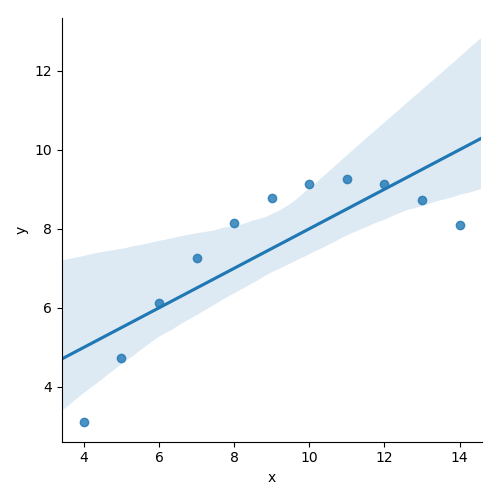
\includegraphics[width=1\textwidth]{gambar13_4}
    \label{fig:13_4}
\end{figure}

Nampaknya data tidak 'pas' untuk dimodelkan dengan regresi linier, maka kita sebagai analis data harus mencoba metode pemodelan non-linier, yakni regresi polinomial orde 2:

\lstinputlisting[language=Python]{contoh13_5.py}
Dan hasilnya dapat dilihat, bahwa model yang kita terapkan sangat sesuai dengan data:
\begin{figure}[H]
    \centering
    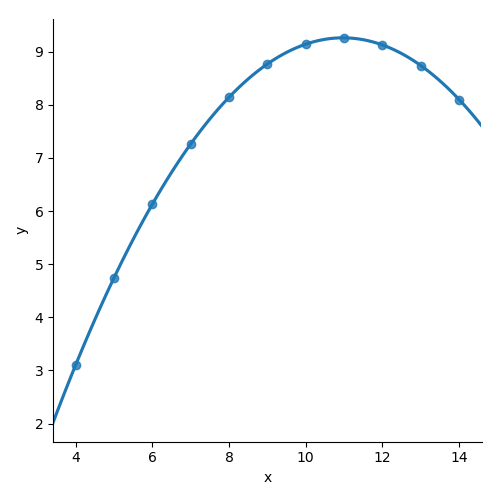
\includegraphics[width=1\textwidth]{gambar13_5}
    \label{fig:13_5}
\end{figure}
\chapter{Visualisasi Matriks}
Terdapat dua jenis visualisasi matriks yang umum digunakan dalam seaborn, yakni \textit{heatmap} dan \textit{clustermap}. Pada bagian ini kita akan membahas keduanya dengan menggunakan dua data bawaan dari seaborn, yakni \verb|tips| dan \verb|flights|. Karena kita belum melihat dataset \verb|flights| yang sebetulnya hanya data bulanan jumlah penumpang pesawat dari tahun 1949 hingga 1960, maka ada baiknya kita lihat dulu datanya:
\lstinputlisting[language=Python]{contoh14_1.py}
Hasilnya adalah:
\lstinputlisting[language={}, numbers=none]{output14_1.txt}
\section{\textit{Heatmap}}
Guna memvisualisasikan data dengan menggunakan \textit{heatmap}, kita memerlukan data yang berformat matriks. Artinya adalah jumlah peubah pada indeks sesuai dengan jumlah peubah pada kolom data. Untuk membentuk bentuk data yang sesuai, kita umumnya menggunakan metode korelasi data atau tabel pivot. Berikut kita akan mencoba dulu dengan menggunakan metode korelasi data pada dataset \verb|tips|:
\lstinputlisting[langauge=Python]{contoh14_2.py}
Inilah tabel korelasi yang dihasilkan:
\lstinputlisting[language={}, numbers=none]{output14_2.txt}
Berikut ini visual \textit{heatmap}-nya:
\begin{figure}[H]
    \centering
    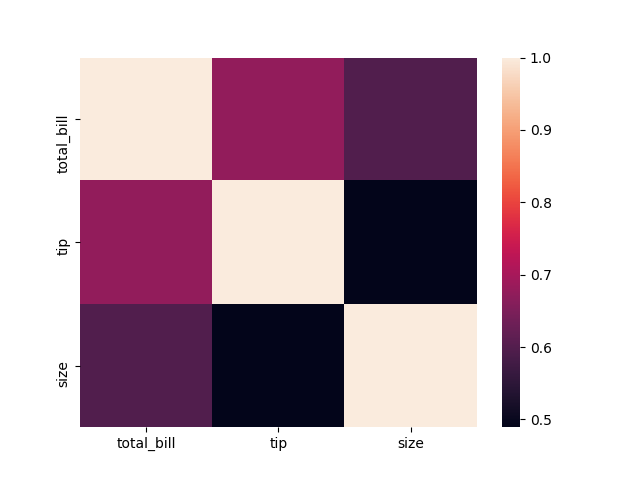
\includegraphics[width=1\textwidth]{gambar14_1}
    \label{fig:14_1}
\end{figure}

Kita juga dapat menampilkan nilai setiap elemen dalam matriks dengan menambahkan argumen \verb|annot=True|, serta mengganti warna pada plot sebagai berikut ini:
\lstinputlisting[language=Python]{contoh14_3.py}
\begin{figure}[H]
    \centering
    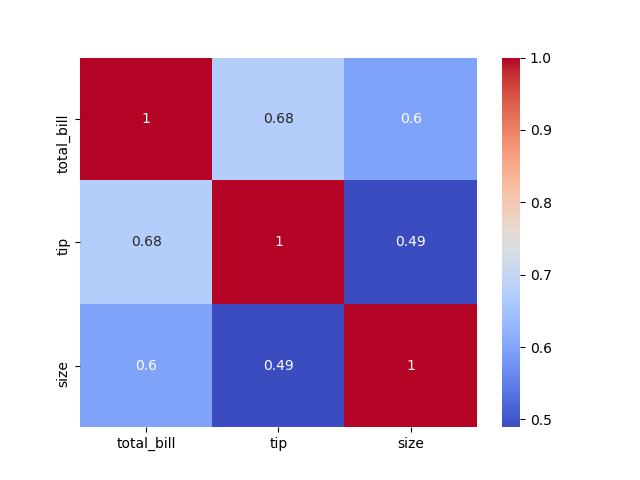
\includegraphics[width=1\textwidth]{gambar14_2}
    \label{fig:14_2}
\end{figure}

Sekarang kita akan mencoba menggunakan tabel pivot (\textit{kan} orang Indonesia pada \textit{jago} pakai \textbf{Excel} jadi ga usah saya \textit{jelasin} lagi hehe). Dalam konteks ini, kita akan menggunakan dataset \verb|flights| dengan menjadikan bulan sebagai baris dan tahun sebagai kolom:
\lstinputlisting[language=Python]{contoh14_4.py}
Berikut ini tabel pivot yang kita hasilkan:
\lstinputlisting[language={}]{output14_3.txt}
Hasil \textit{heatmap}-nya adalah sebagai berikut:
\begin{figure}[H]
    \centering
    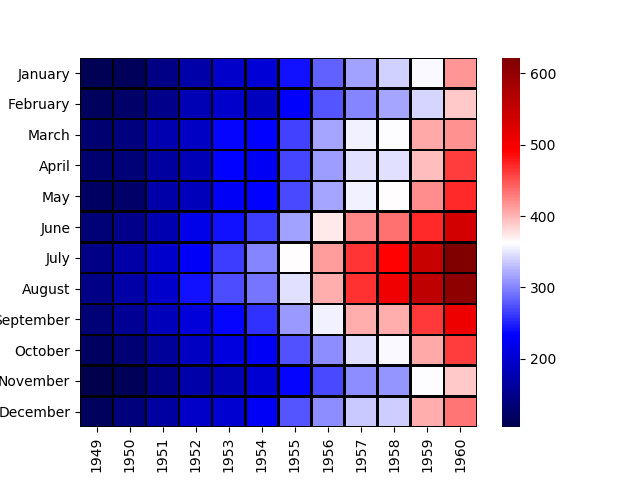
\includegraphics[width=1\textwidth]{gambar14_3}
    \label{fig:14_3}
\end{figure}

Melalui grafik di atas, kita dapat melihat bahwa jumlah penumpang pesawat paling banyak pada bulan - bulan musim panas di belahan bumi utara (karena konteks data ini mengambil contoh kasus di Amerika Serikat) dan semakin bertambah banyak seiring dengan proses keberjalanan waktu.

\section{\textit{Clustermap}}
Untuk melanjukan proses analisis pengelompokan jumlah penumpang pesawat berdasarkan bulan dan tahun pada contoh di atas, kita dapat menerapkan \href{https://en.wikipedia.org/wiki/Hierarchical_clustering}{\textbf{algoritma \textit{clustering} hierarkis}} dan memvisualisasikannya dengan menggunakan \textit{clustermap} seperti contoh berikut ini: 
\lstinputlisting[language=Python]{contoh14_5.py}
\begin{figure}[H]
    \centering
    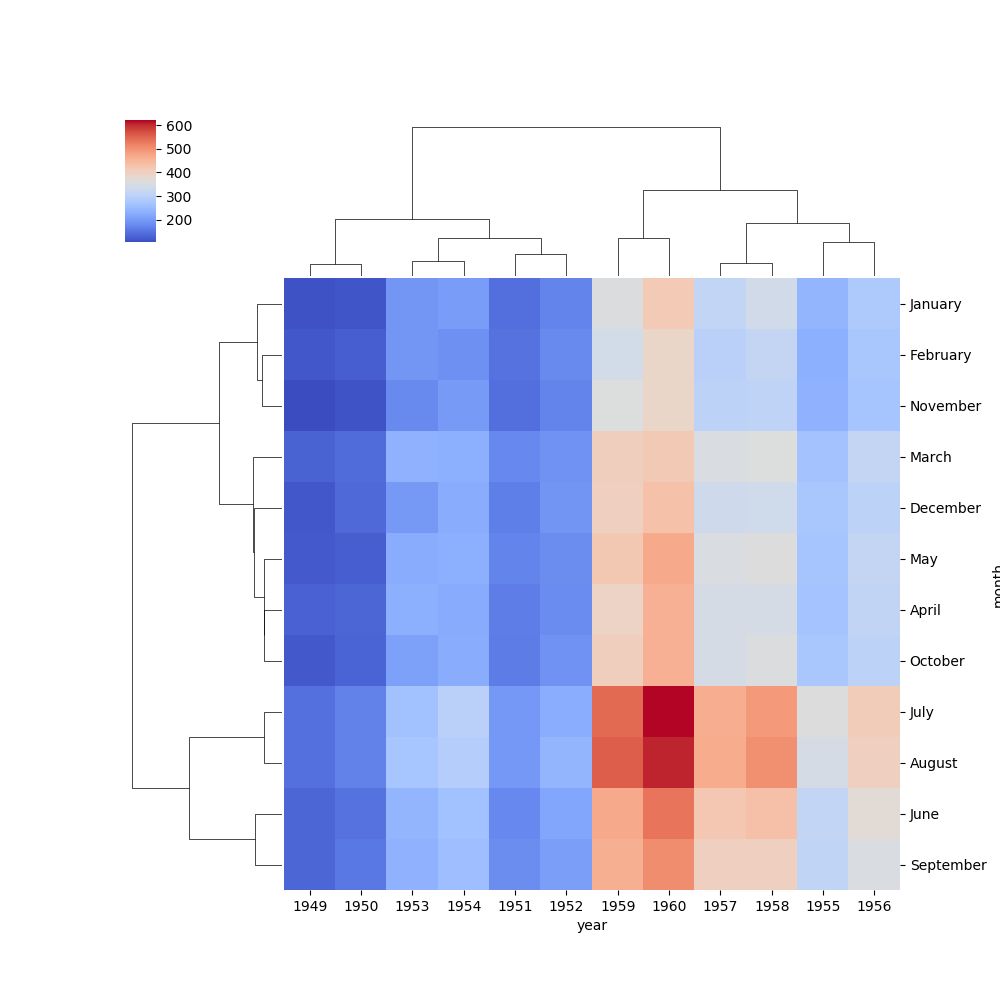
\includegraphics[width=1\textwidth]{gambar14_4}
    \label{fig:14_4}
\end{figure}
Karena skalanya masih dalam skala jumlah penumpang pesawat, kita dapat memperjelasnya dengan melakukan standarisasi skala dari 0 hingga 1:
\lstinputlisting[language=Python]{contoh14_6.py}
\begin{figure}[H]
    \centering
    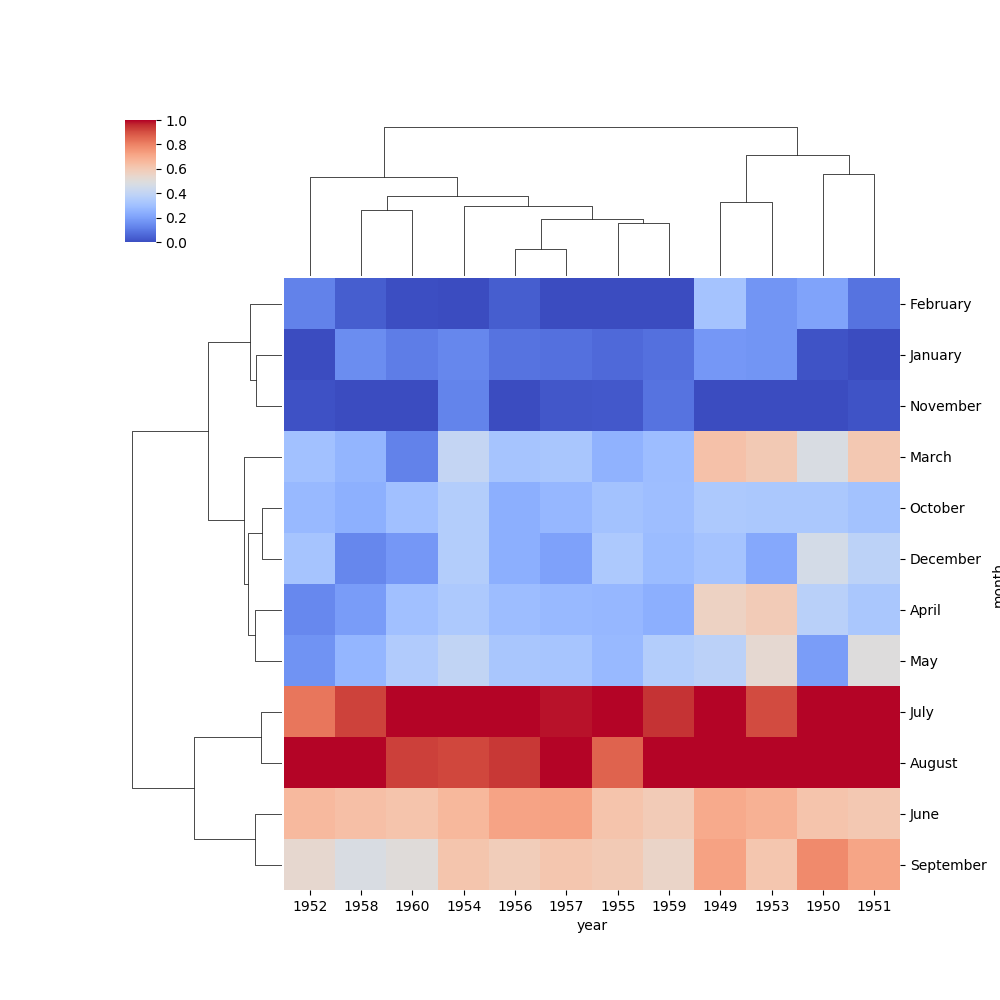
\includegraphics[width=1\textwidth]{gambar14_5}
    \label{fig:14_5}
\end{figure}

Perhatikanlah bahwa kini tahun dan bulan pada grafik tidak lagi berurutan, melainkan dikelompokan berdasarkan kesamaan jumlah penumpangnya. Nampak kemiripan antara bulan Juli dan Agustus sebagai bulan dengan jumlah penumpang terbanyak, dan hal ini masuk akal karena sedang berlangsung liburan musim panas di Amerika pada bulan - bulan itu.
\end{document}
